\chapter{Auswertung}
\label{auswertung}
Im Rahmen dieses Kapitels werden in einem ersten Schritt Neo4j und die beiden Db2 Graph Versionen anhand der Messergebnisse aus \autoref{ergebnisse} eingeordnet und miteinander verglichen. Dabei werden auch Kennzahlen ermittelt, die verdeutlichen, wie groß die Performance-Unterschiede zwischen ihnen sind. 

Anschließend wird untersucht welchen Einfluss die Faktoren Größe der Ergebnismenge und Datensatzgröße auf die Performance der Systeme haben. Darüber hinaus werden auch die von NMON erstellten Ressourcenstatistiken, die während den Messungen aufgezeichnet werden, in begrenztem Umfang ausgewertet. Zusätzlich werden in diesem Abschnitt auch die von Db2 Graph generierten SQL-Anweisungen genauer untersucht, um herauszufinden, was die Ursache für den großen Performance-Unterschied zwischen den Db2 Graph Versionen ist.

Dabei gilt es anzumerken, dass in diesem Kapitel hauptsächlich der Durchsatz als Indikator für Performance herangezogen wird. Dies wird damit begründet, dass im Kontext von \autoref{ergebnisse} der Fokus bei der Besprechung der Ergebnisse hauptsächlich auf der Latenz liegt.

\section{Einordnung und Vergleich der Performance}
\label{auswertung:einordnung}
Bei der Beurteilung der Performance der Datenbanksysteme handelt es sich bei den im Rahmen der Arbeit erzielten Messergebnissen um eine einfache Aufgabe. So weist bei jeder Messreihe Neo4j den niedrigsten Latenz- und Durchsatzwert auf, gefolgt von Db2 Graph Beta 3 -- sollte es Teil der Messreihe sein -- und Db2 Graph V11.5.6.0. 

Bei dem Vergleich der in der Messreihe beschriebenen Ergebnisse fällt zugleich auf, dass es sich hierbei nicht um einen kleinen Unterschied zwischen den jeweiligen Datenbanksystemen handelt. So scheinen sich die Datenbanksysteme sowohl bei der durchschnittlichen Latenz als auch bei dem Durchsatz um einen ähnlichen Faktor zu unterscheiden. Um die Datenbanksysteme bezüglich ihrer Performance einordnen und vergleichen zu können, wäre ein solcher Performance-Faktor ein passendes Maß. 

Um eine dementsprechende Kennzahl zur Einordnung der Datenbanksysteme bezüglich ihrer Performance bereitstellen zu können, wird daher ein gemeinsamer Durchschnittswert für den Durchsatz der Operationen:
\begin{itemize}
    \item \texttt{getNode}
    \item \texttt{getLink}
    \item \texttt{countLink} und 
    \item \texttt{getLinkList} (Range-Limit 100) ermittelt.
\end{itemize}
Der gemeinsame Durchschnittswert für den Durchsatz wird dabei einmal für jedes Datenbanksystem im Kontext einer Messreihe ermittelt. Anschließend wird der niedrigste Wert einer Messreihe herangezogen -- immer Db2 Graph V11.5.6.0 -- und als Faktor 1 festgelegt. Im nächsten Schritt werden, basierend auf diesem Faktor 1 und dem damit verbundenen Durchschnittswert, die jeweiligen Faktoren für Neo4j und gegebenenfalls Db2 Graph Beta 3 errechnet. Die dabei erhaltenen Performance-Faktoren -- basierend auf dem Durchsatz -- werden für die Messreihen mit einem konstant verteilten Datensatz in \autoref{fig:faktor:durchsatz:const} dargestellt, während die mit real verteilten Datensätzen in \autoref{fig:faktor:durchsatz:real} abgebildet werden.

\begin{figure}[!ht]
    \centering
    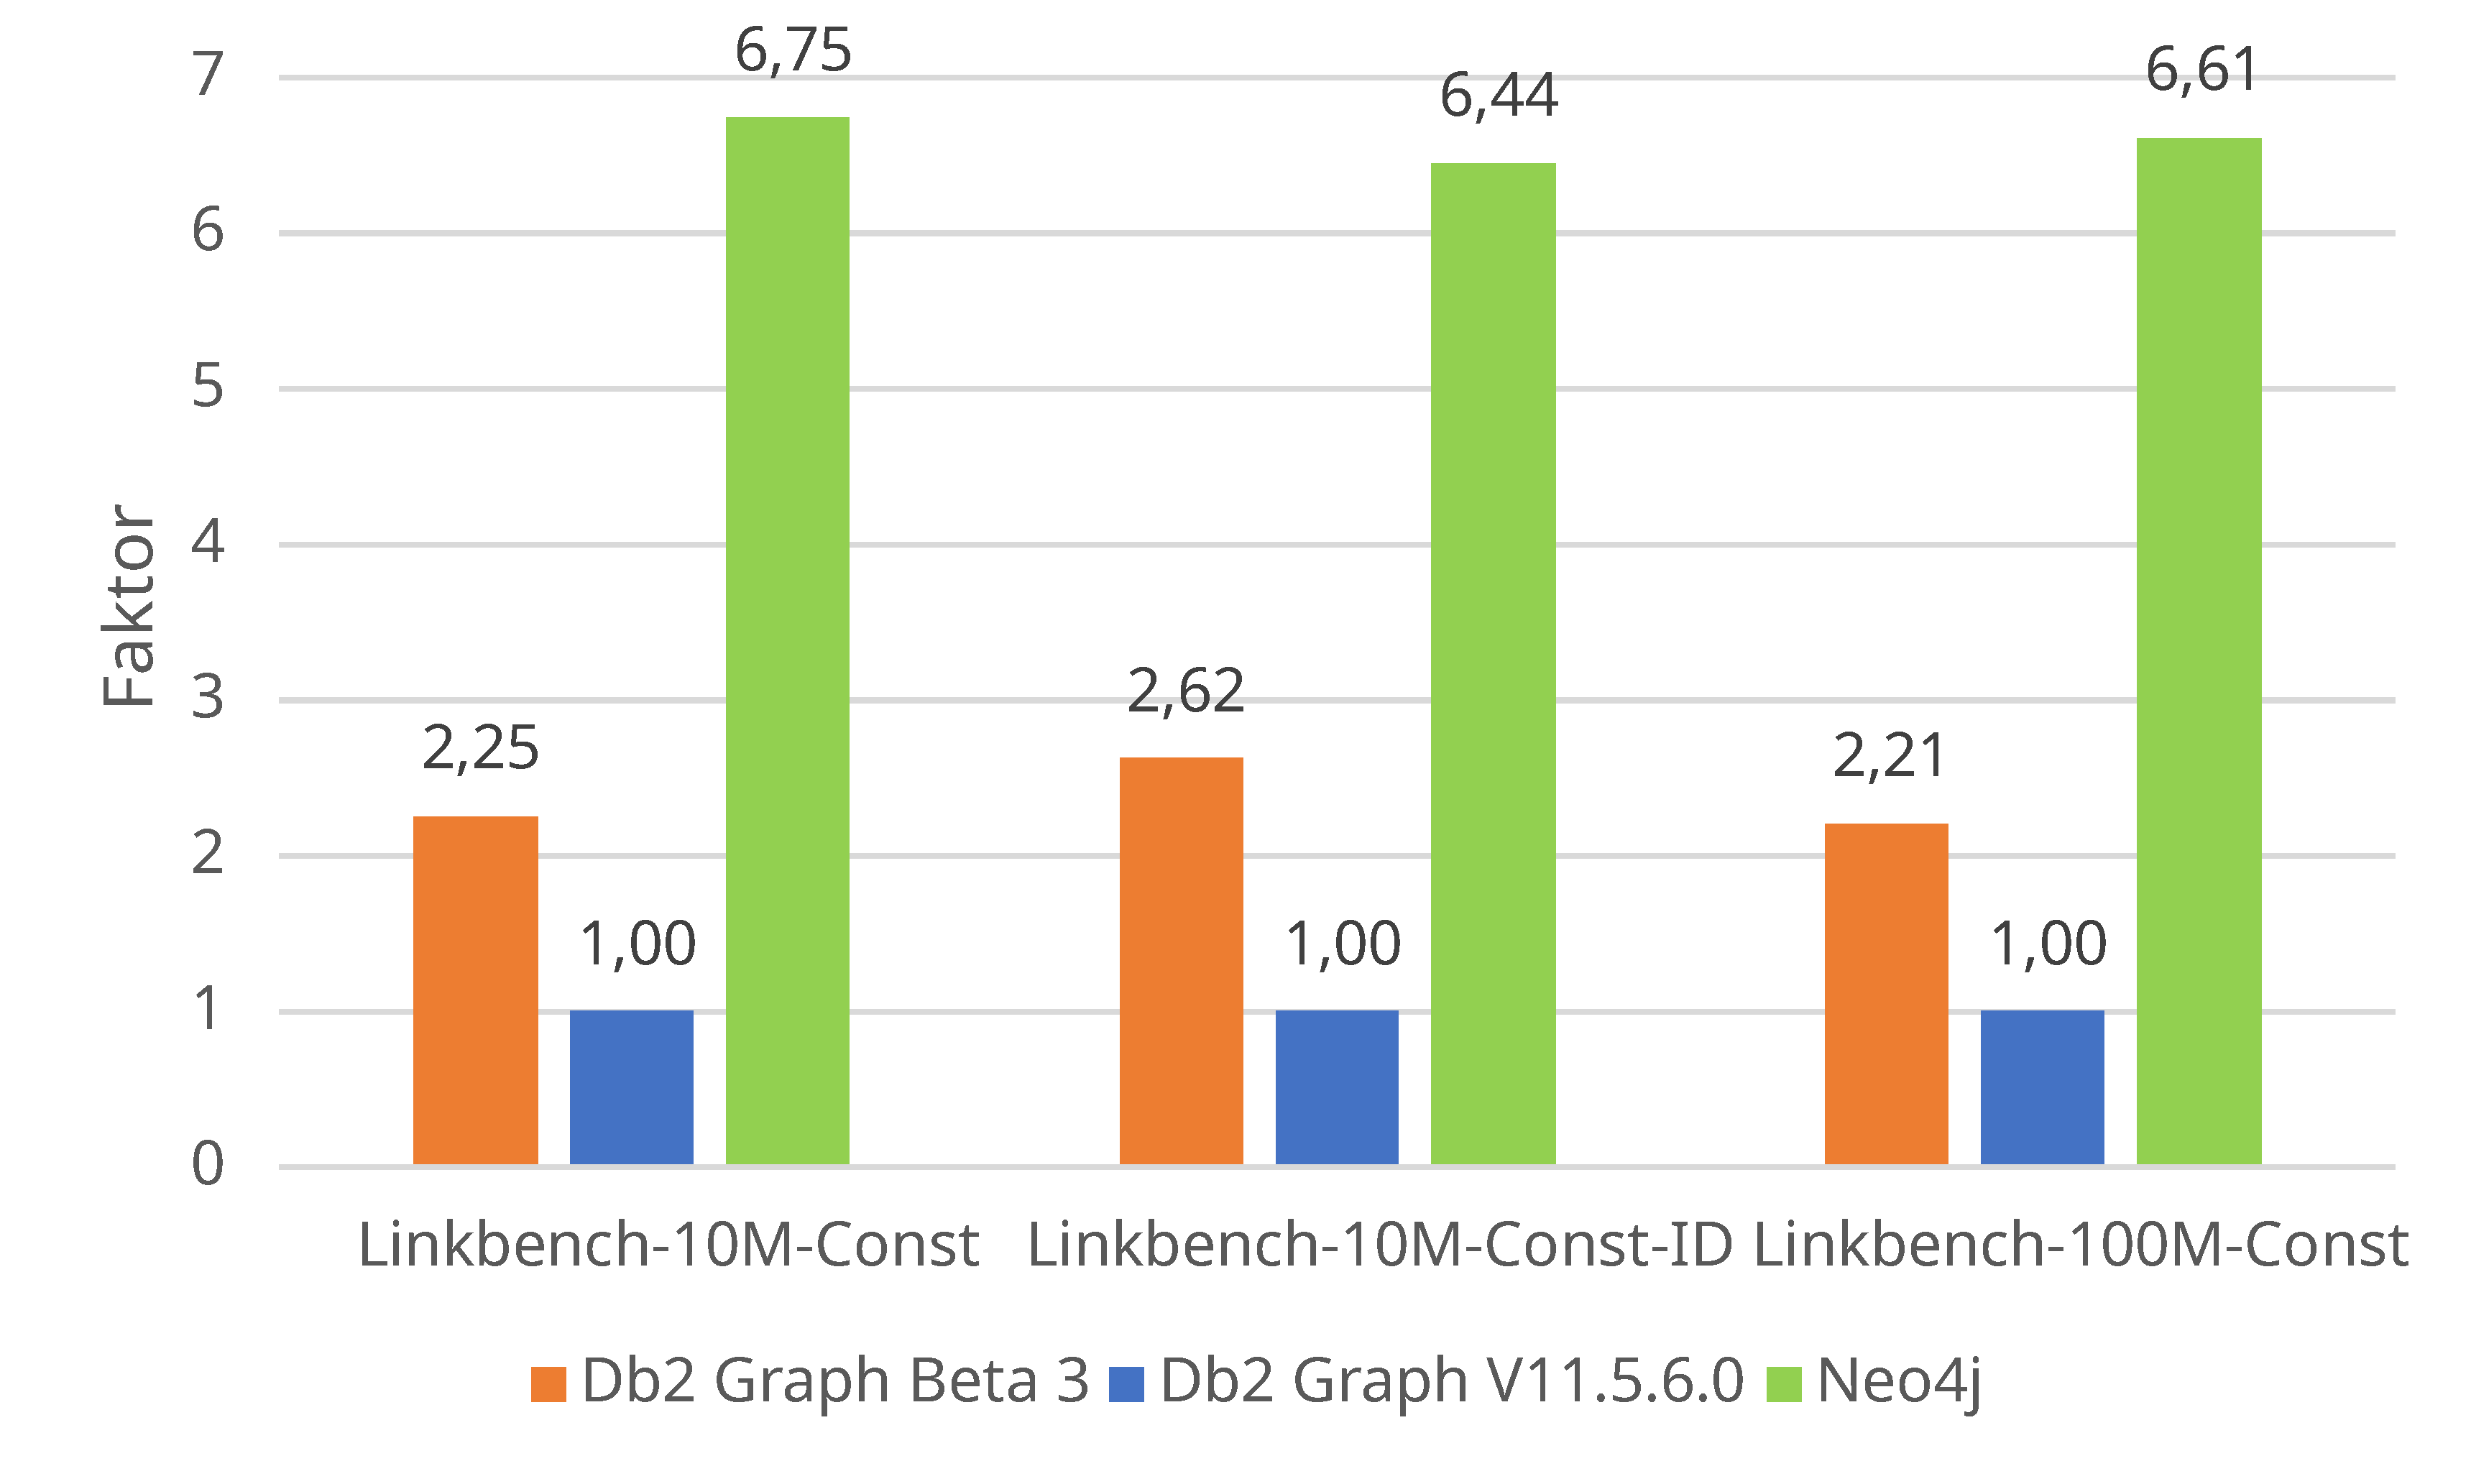
\includegraphics[width=\textwidth]{images/diagramme/faktor_durchschittlicher_durchsatz_const.pdf}
    \caption{Performance-Faktor bei Messreihen mit konstant verteilten Datensätzen}
    \label{fig:faktor:durchsatz:const}
\end{figure}

\begin{figure}[!ht]
    \centering
    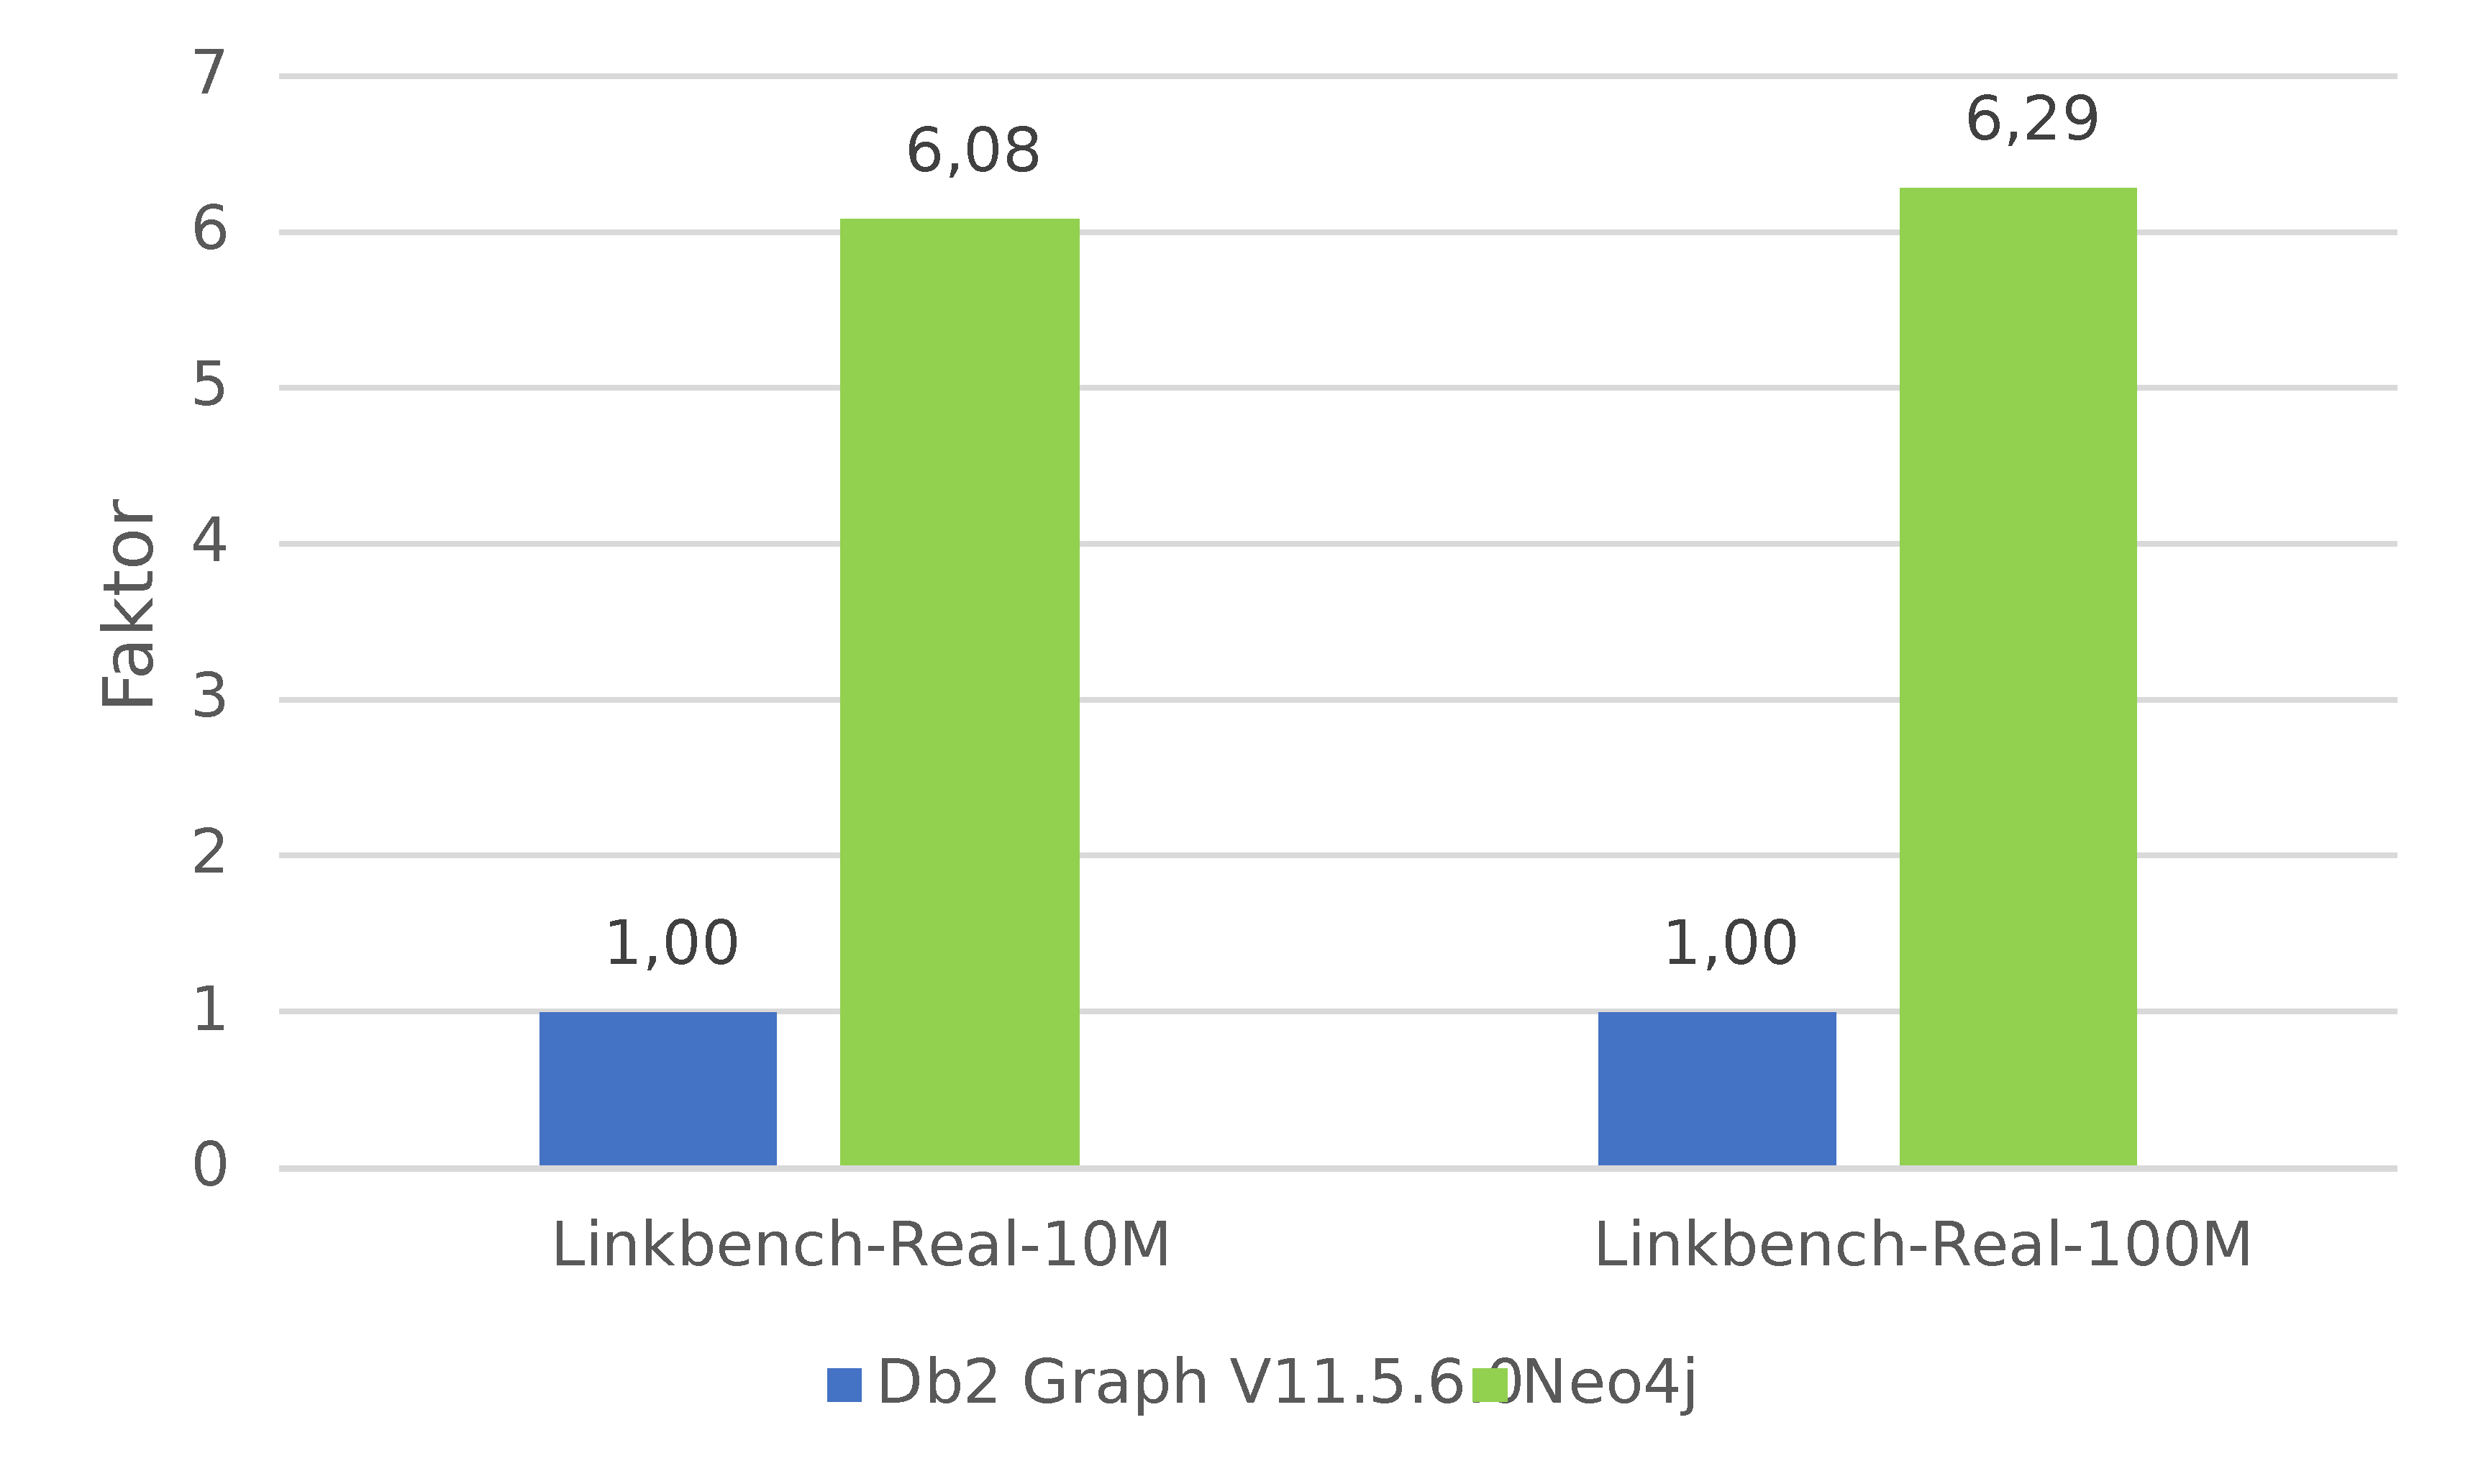
\includegraphics[width=\textwidth]{images/diagramme/faktor_durchschittlicher_durchsatz_real.pdf}
    \caption{Performance-Faktor bei Messreihen mit real verteilten Datensätzen}
    \label{fig:faktor:durchsatz:real}
\end{figure}

Bei der Analyse der in \autoref{fig:faktor:durchsatz:const} und \ref{fig:faktor:durchsatz:real} dargestellten Faktoren fällt auf, dass Neo4j immer sechs bis siebenmal so viele Operationen pro Sekunde verarbeitet wie Db2 Graph V11.5.6.0. Dies offenbart einen erheblichen Performance-Unterschied zwischen Db2 Graph V11.5.6.0 und Neo4j. Während Db2 Graph Beta 3 zwar mit einem Faktor von 2,25 eine höhere Performance aufweist als V11.5.6.0, verfügt es lediglich über ca. ein Drittel der Performance von Neo4j (\autoref{fig:faktor:durchsatz:const}).  

So war von Beginn an nicht davon auszugehen, dass Db2 Graph als Grapherweiterung in Kombination mit Db2, Neo4j als natives Graphdatenbanksystem übertrifft. Schließlich verursacht die Kommunikation zwischen Db2 Graph und Db2, die für die Beantwortung einer Anfrage nötig ist, einen Aufwand, den Neo4j nicht betreiben muss. Einen Performance-Unterschied um mindestens den Faktor 6 wurde jedoch nicht erwarten. 

Eine interessante Gegebenheit, die in der \autoref{fig:faktor:durchsatz:const} beobachtet werden kann, stellt der Fakt dar, dass Db2 Graph Beta 3 als ältere Version von Db2 Graph 2 bis 2,5 Mal mehr Operationen pro Sekunde bewältigen kann, als Db2 Graph V11.5.6.0 (der erste \acs{ga} Release). Zu Beginn wäre hier eigentlich die Vermutung nahe gelegen, dass V11.5.6.0 als neuere Version, die über mehr Optimierungen verfügt als Beta 3, eine höhere Performance aufweist. Dies ist allerdings nicht der Fall. 

Dabei gilt es hingegen zu beachten, dass Db2 Graph Beta 3 trotz der höheren Performance bei den Messreihen mit konstant verteilten Datensätzen, nicht als allgemein performantere Version von Db2 Graph einzustufen ist. Schließlich spielt sie bei den Messreihen mit real verteilten Datensätzen keine Rolle, da sie für den Einsatz dort aufgrund fehlender Optimierungen derart ungeeignet ist, dass das Erzielen von Ergebnissen im Rahmen des üblichen Zeitraums nicht möglich ist.

\section{Umgang mit Ergebnismengen}
\label{auswertung:ergebnismenge}
Bei der Untersuchung der Ergebnismenge bei den Messreihen mit real verteilten Datensätzen wird bereits in \autoref{ergebnisse:10m_real} und \ref{ergebnisse:100m_real} ein kurzer Überblick über das jeweilige Verhalten bezüglich des Durchsatzes gegeben. Wie groß der verhältnismäßige Einbruch des Durchsatzes und entsprechend auch der Performance, bei einer variierenden oberen Grenze für die Anzahl an Elementen in einer Ergebnismenge ist, lässt sich an den Abbildungen, die absolute Zahlen präsentieren, nicht ablesen. Schließlich bewegen sich die Datenbanksysteme mit beispielsweise 15.742 und 2.466 Operationen pro Sekunde in \autoref{ergebnisse:10m_real} in anderen Größenordnungen, werden aber in derselben Grafik abgebildet. 

Um nun der Frage auf den Grund zugehen: \textit{Welches Datenbanksystem bei einem steigenden Range-Limit den verhältnismäßig größeren Performance-Einbruch aufweist?}, wird in \autoref{fig:einbruch:durchsatz:10m} und \ref{fig:einbruch:durchsatz:100m} dargestellt, wie viel Prozent des Durchsatzes bei einem steigenden Range-Limit noch erreicht werden können. Der Wert für \texttt{getLinkList} mit einem Range-Limit von 100 repräsentiert dabei jeweils 100 \% des Durchsatzes von Neo4j oder Db2 Graph. So sinkt beispielsweise der Durchsatz bei Neo4j in \autoref{fig:einbruch:durchsatz:10m} bei einem Range-Limit von 10.000 auf lediglich 69,74~\% des bei einem Range-Limit von 100 erzielten Durchsatzes. 

Bei der Betrachtung des Kurvenverlaufs in \autoref{fig:einbruch:durchsatz:10m} und \ref{fig:einbruch:durchsatz:100m} fällt auf, dass der Rückgang des Durchsatzes bei Neo4j eher linear ausfällt, während er sich bei Db2 Graph eher exponentiell gestaltet. Für eine endgültige Einstufung der Kurven von Db2 Graph als exponentiell fehlen allerdings einige Mess- beziehungsweise Datenpunkte.

Des Weiteren ist erkennbar, dass der Performance-Einbruch bei Db2 Graph V11.5.6.0 bei einem steigenden Range-Limit immer geringer zu sein scheint als bei Neo4j. So weist V11.5.6.0 bei einem Range-Limit von 100.000 noch 54,18 \% des Durchsatzes auf den es bei einem Range-Limit von 100 erreicht hat. Neo4j hingegen erlangt bei 100.000 lediglich 43,29 \% des Durchsatzes den es erreicht, wenn die Ergebnismenge auf eine obere Grenze von 100 Elemente begrenzt wird. 

So beträgt der Unterschied zwischen Db2 Graph und Neo4j bei einem Range-Limit von 100.000 ca. 11 \% zueinander in \autoref{fig:einbruch:durchsatz:10m}, während es bei 10.000 sogar ca. 18 \% sind. Bei einem Range-Limit von 1.000 sind es jedoch lediglich ca. 8 \% Unterschied zueinander. Wobei es hier anzumerken gilt, dass Db2 Graph mit 97,58~\% ein außergewöhnlich hohes Ergebnis erreicht. Die in \autoref{fig:einbruch:durchsatz:100m} dargestellten Werte bestätigen dabei grob die Beobachtungen aus \autoref{fig:einbruch:durchsatz:10m}. So weichen die Werte in den beiden Abbildungen (\autoref{fig:einbruch:durchsatz:10m} und \ref{fig:einbruch:durchsatz:100m}) maximal um 2 \% voneinander ab. 

\begin{figure}[!ht]
    \centering
    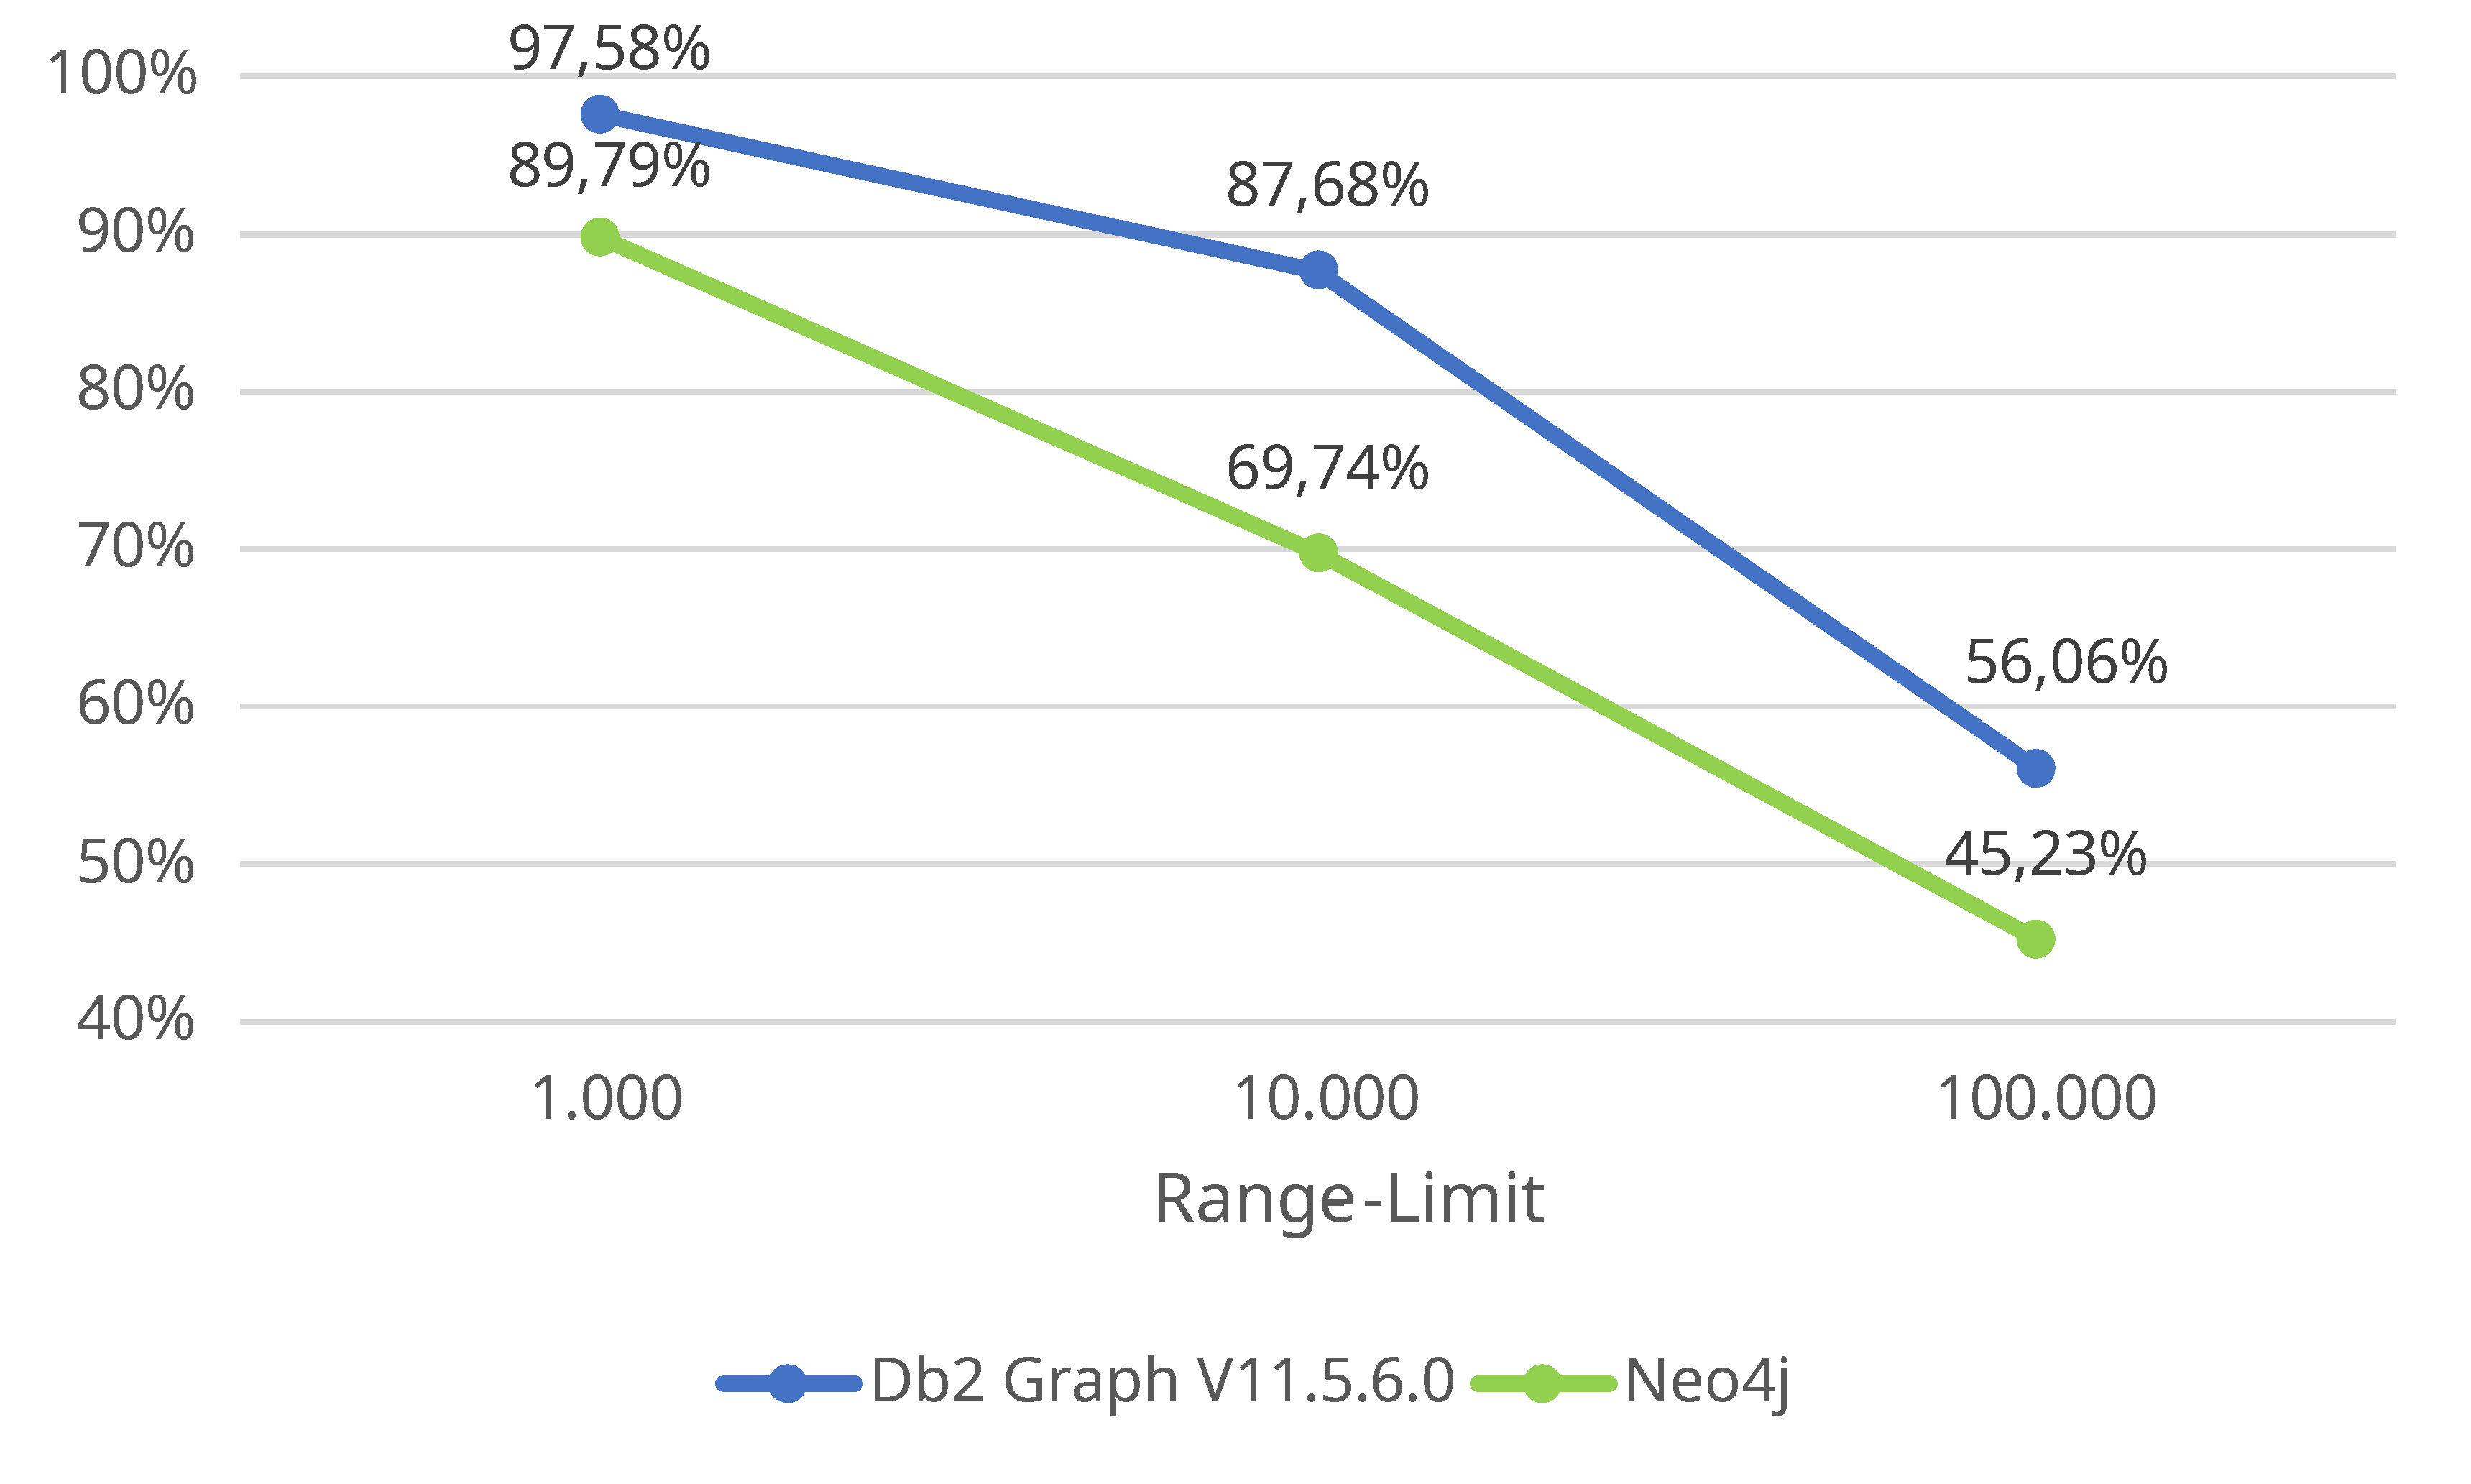
\includegraphics[width=\textwidth]{images/diagramme/limit_relative_durchsatz_real_10m.pdf}
    \caption{Linkbench-Real-10M Durchsatz gemessen an getLinkList(100)}
    \label{fig:einbruch:durchsatz:10m}
\end{figure}

\begin{figure}[!ht]
    \centering
    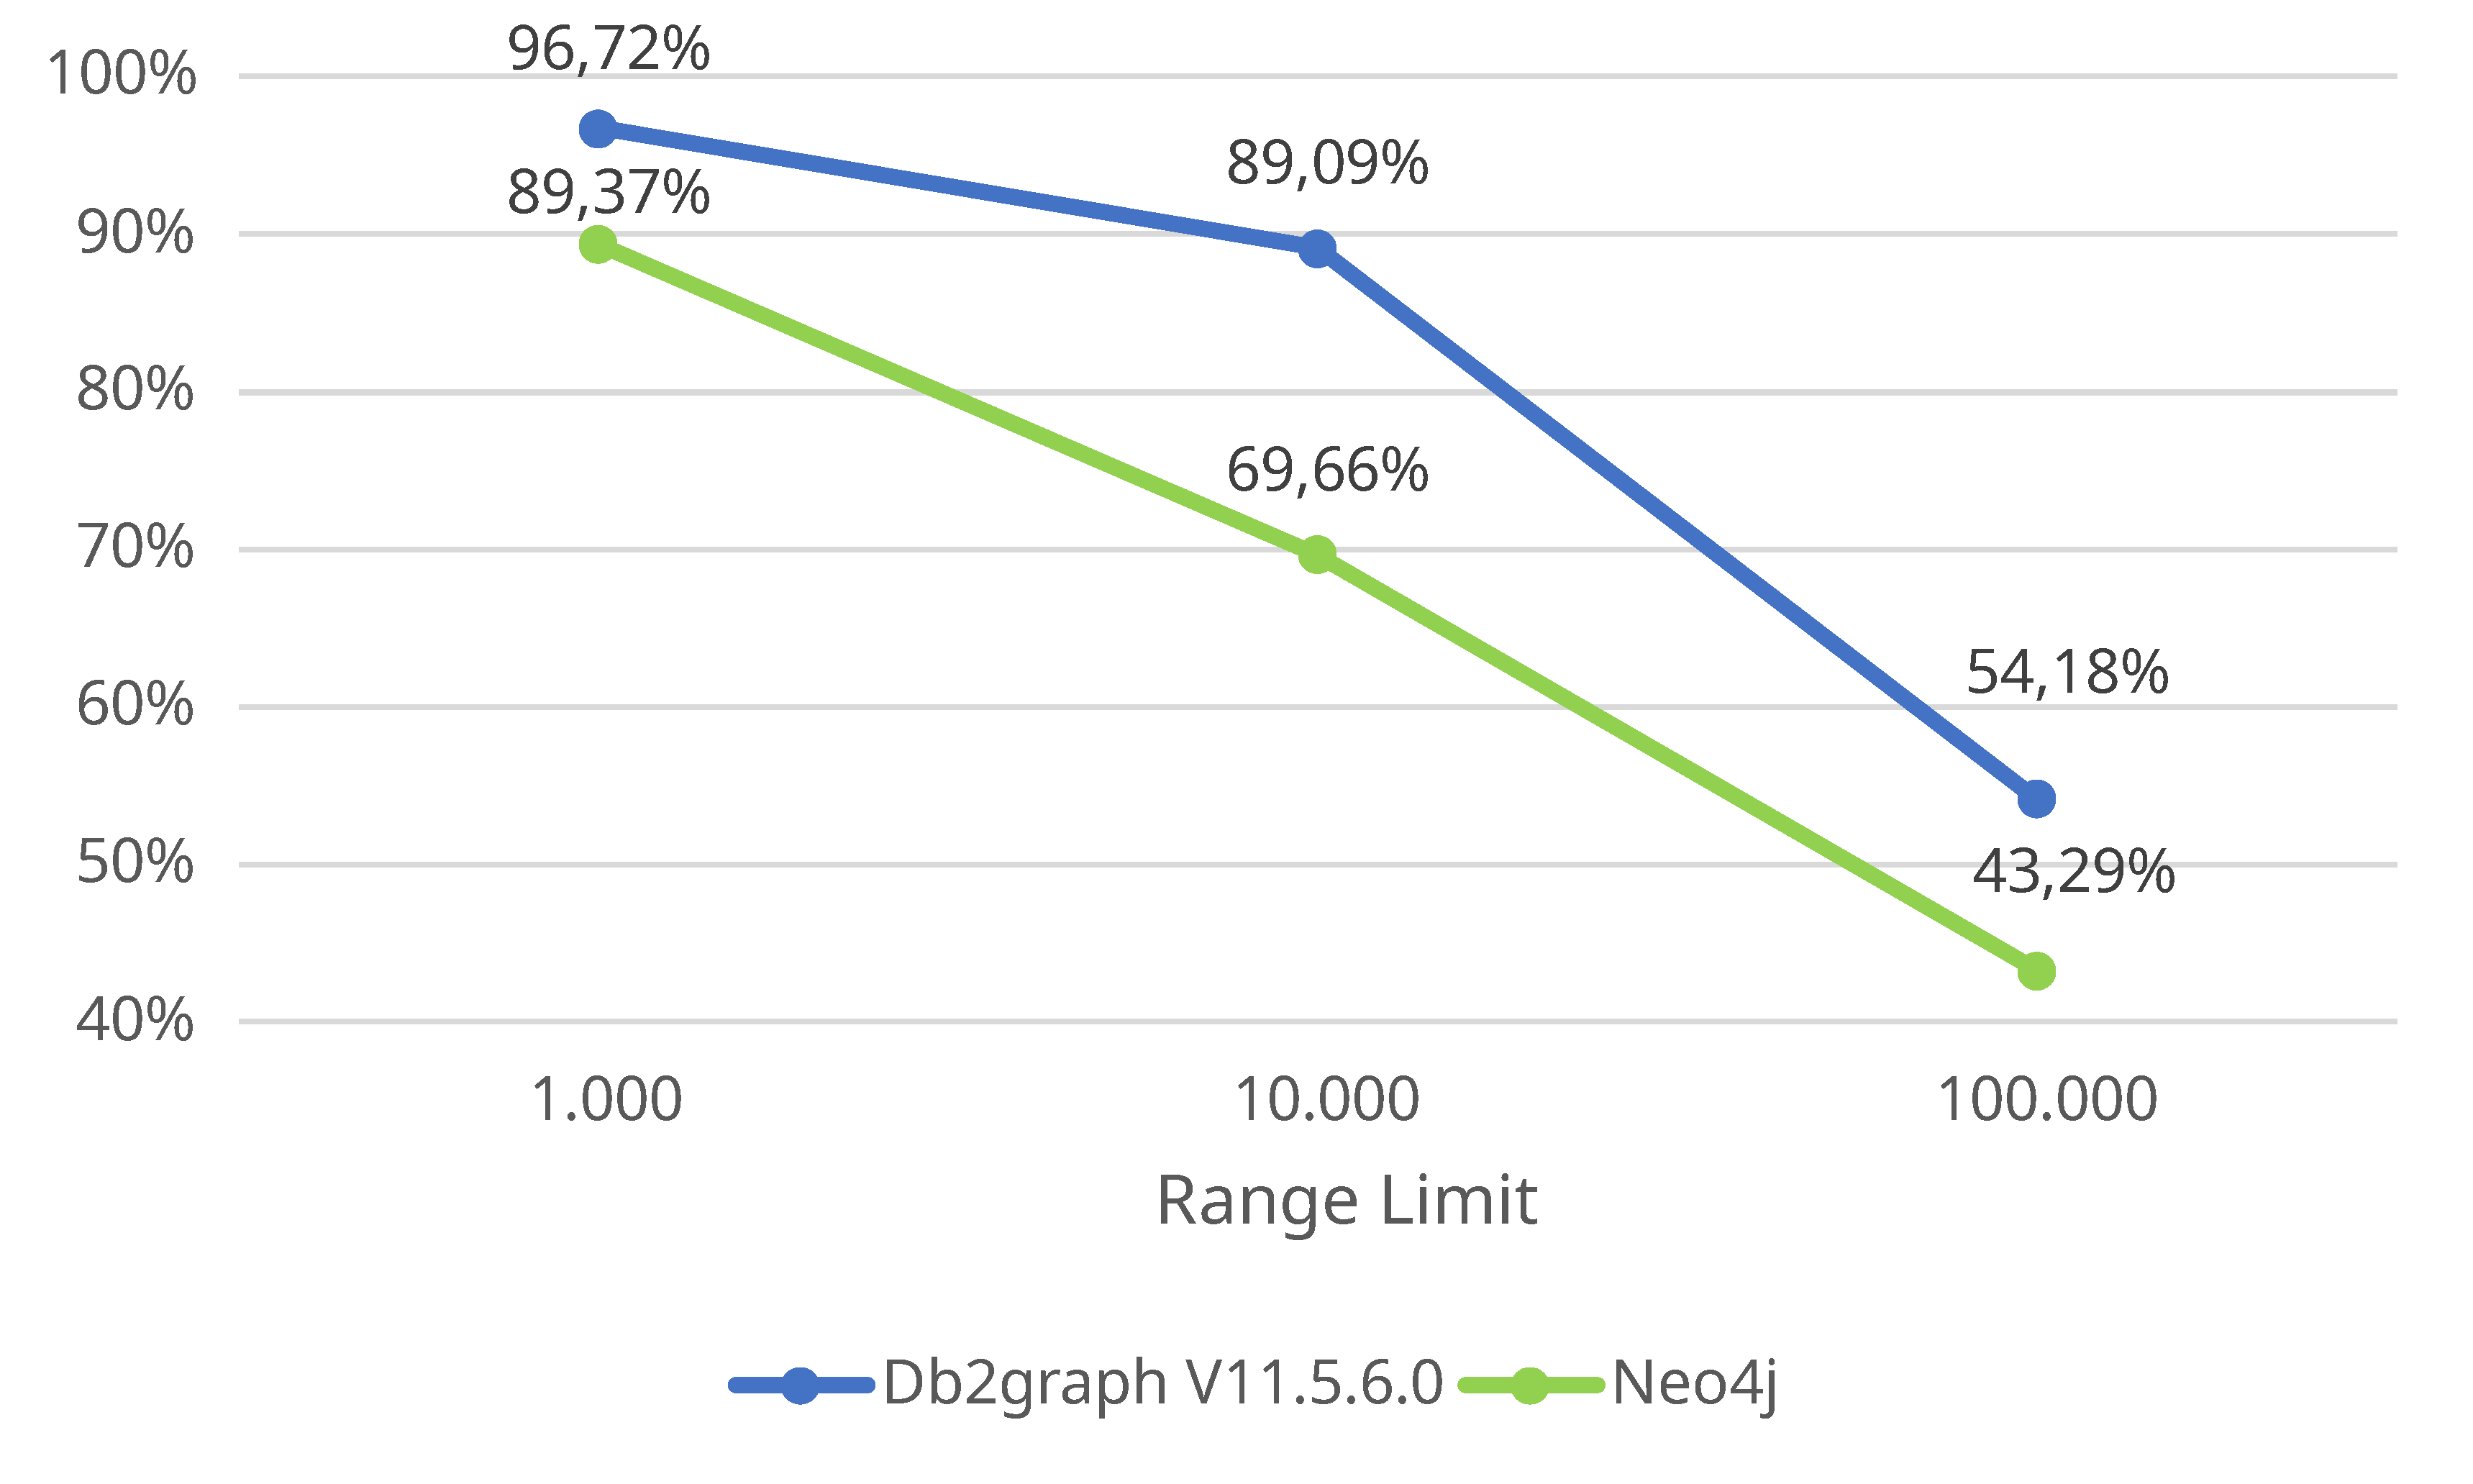
\includegraphics[width=\textwidth]{images/diagramme/limit_relative_durchsatz_real_100m.pdf}
    \caption{Linkbench-Real-100M Performance gemessen an getLinkList(100)}
    \label{fig:einbruch:durchsatz:100m}
\end{figure}

Basierend auf \autoref{fig:einbruch:durchsatz:10m} und \ref{fig:einbruch:durchsatz:100m} kann das Fazit gezogen werden, dass der Performance-Einbruch von Neo4j bei dem Umgang mit größeren Ergebnismengen nicht nur in absoluten Zahlen, sondern auch im Verhältnis, etwas höher ausfällt als bei Db2 Graph. 

Allerdings bewegt sich Neo4j dauerhaft auf einem höheren Niveau als Db2 Graph, wodurch Neo4j auch noch bei einem Range-Limit von 100.000 in absoluten Zahlen einen höheren Durchsatz beziehungsweise eine höhere Performance erzielt als Db2 Graph V11.5.6.0 (siehe \autoref{fig:durchsatz:linkbench_10m_real:rl} und \ref{fig:durchsatz:linkbench_100m_real:rl}).

\section{Einfluss der Datensatzgröße}
\label{auswertung:groesse}
Im Rahmen dieses Abschnitts wird genauer untersucht, welchen Einfluss die Größe eines Datensatzes auf konstant oder real verteilte Datensätze hat. Um dies bei den Datenbanksystemen zu identifizieren, wird der relative Unterschied zwischen den Durchsatzergebnissen von Linkbench-10M und Linkbench-100M Datensätzen ermittelt. Die jeweiligen Durchsatzergebnisse, die mit Linkbench-10M Datensätzen erzielt werden, werden dabei als 100~\% betrachtet. An diesen 100~\% wird im nächsten Schritt der Durchsatz bei den Linkbench-100M Datensätzen gemessen. Die prozentualen Abweichungen zwischen den Datensätzen werden dabei in \autoref{fig:durchsatz:10m_vs_100m:const} und \ref{fig:durchsatz:10m_vs_100m:real} dargestellt.

\begin{figure}[!ht]
    \centering
    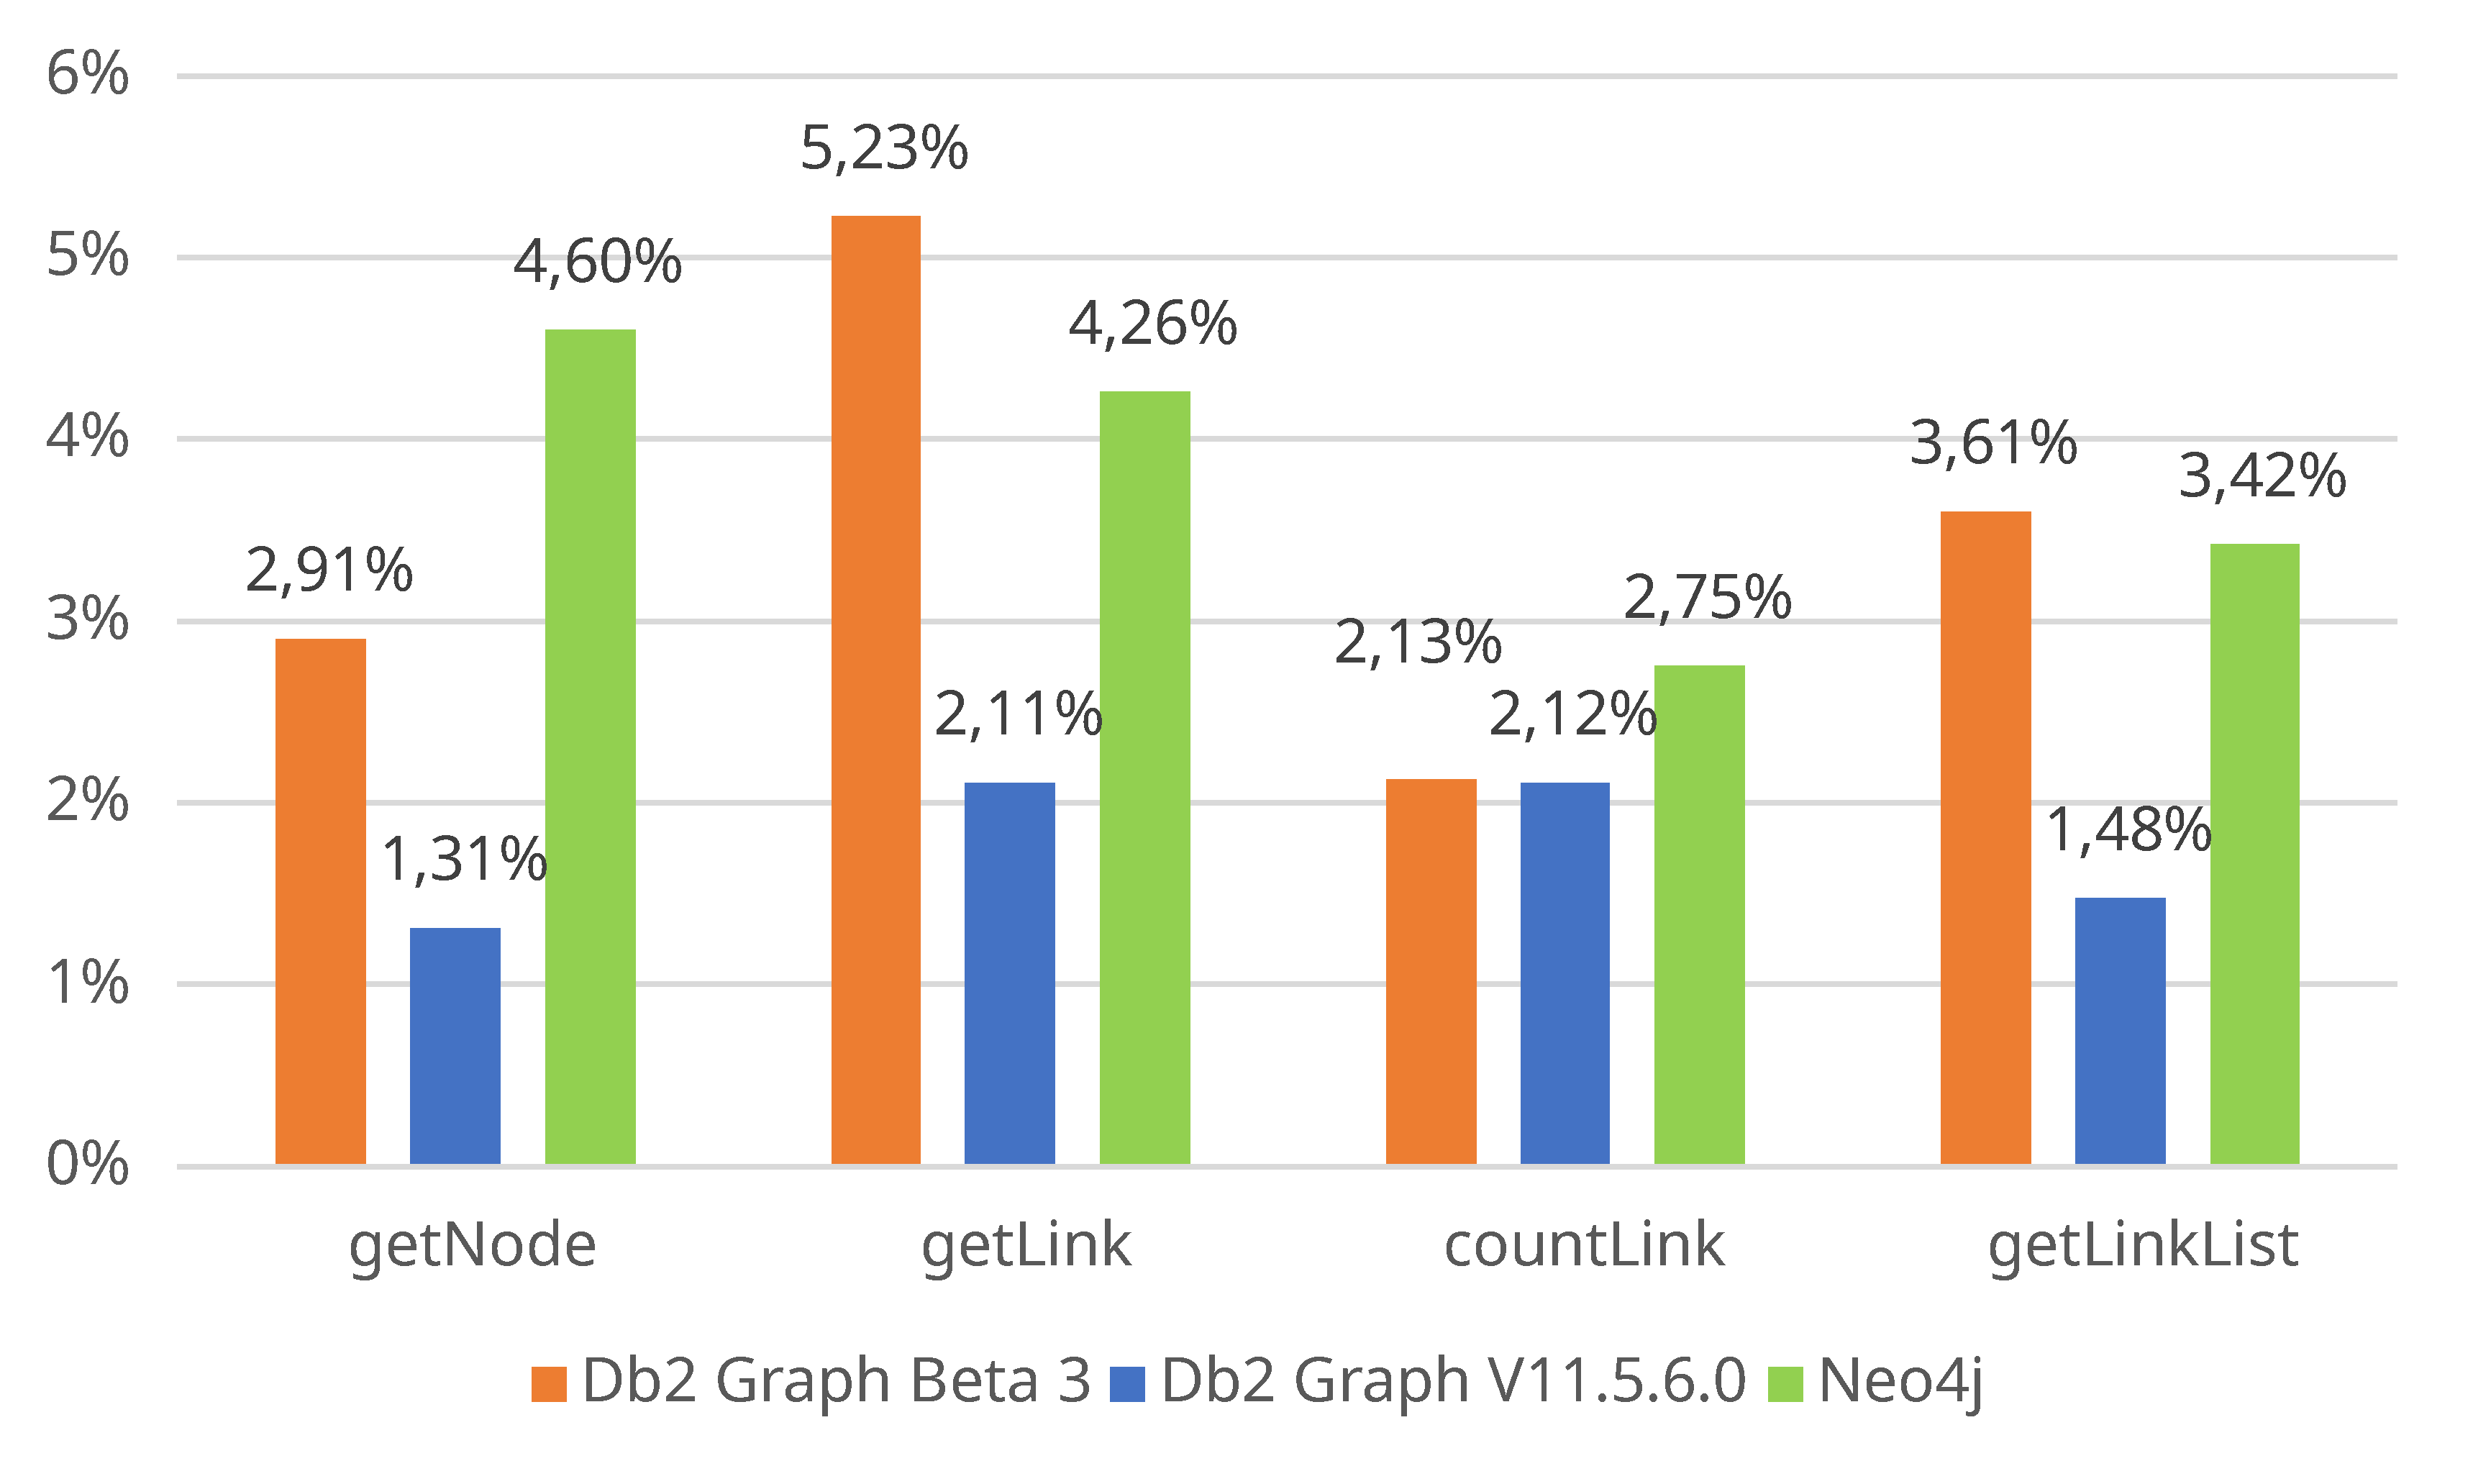
\includegraphics[width=\textwidth]{images/diagramme/difference_durchsatz_const_10m_vs_100m.pdf}
    \caption{Unterschied Durchsatz Linkbench-10M vs. Linkbench-100M (Const)}
    \label{fig:durchsatz:10m_vs_100m:const}
\end{figure}

Es gilt den in \autoref{fig:durchsatz:10m_vs_100m:const} bei \texttt{getNode} für Db2 Graph Beta 3 angegebenen Wert von 2,91 \% so zu verstehen, dass der Durchsatz bei Linkbench-100M um diesen Prozentsatz geringer ausfällt als bei derselben Messung mit dem Linkbench-10M. Db2 Graph Beta 3 erreicht also bei der Messreihe \nameref{ergebnisse:100m_const} lediglich 97,09 \% des Durchsatzes von der Messreihe \nameref{ergebnisse:10m_const}, wodurch sich der Unterschied von 2,91 \% bei \texttt{getNode} ergibt.

Die in \autoref{fig:durchsatz:10m_vs_100m:const} für konstant verteilte Datensätze dargestellten Ergebnisse zeigen hier ein konstantes Bild über alle Datenbanksysteme hinweg. So weisen alle Messergebnisse, egal welches Datenbanksystem oder welche Operation, eine positive prozentuale Abnahme auf. Dies bedeutet, dass -- wie bei größeren Datensätzen erwartet -- alle Durchsatzergebnisse von \nameref{ergebnisse:100m_const} im Verhältnis zu \nameref{ergebnisse:10m_const} niedriger ausfallen. Db2 Graph V11.5.6.0 weist dabei mit 1,31 \% bis 2,12 \% den geringsten Performance-Einbruch auf. Neo4j und Db2 Graph Beta 3 hingegen verfügen über deutlich höhere Performance-Einbrüche bei dem größeren Datensatz mit jeweils 4,60 \% (\texttt{getNode}) und 5,23 \% (\texttt{getLink}). 

\begin{figure}[!ht]
    \centering
    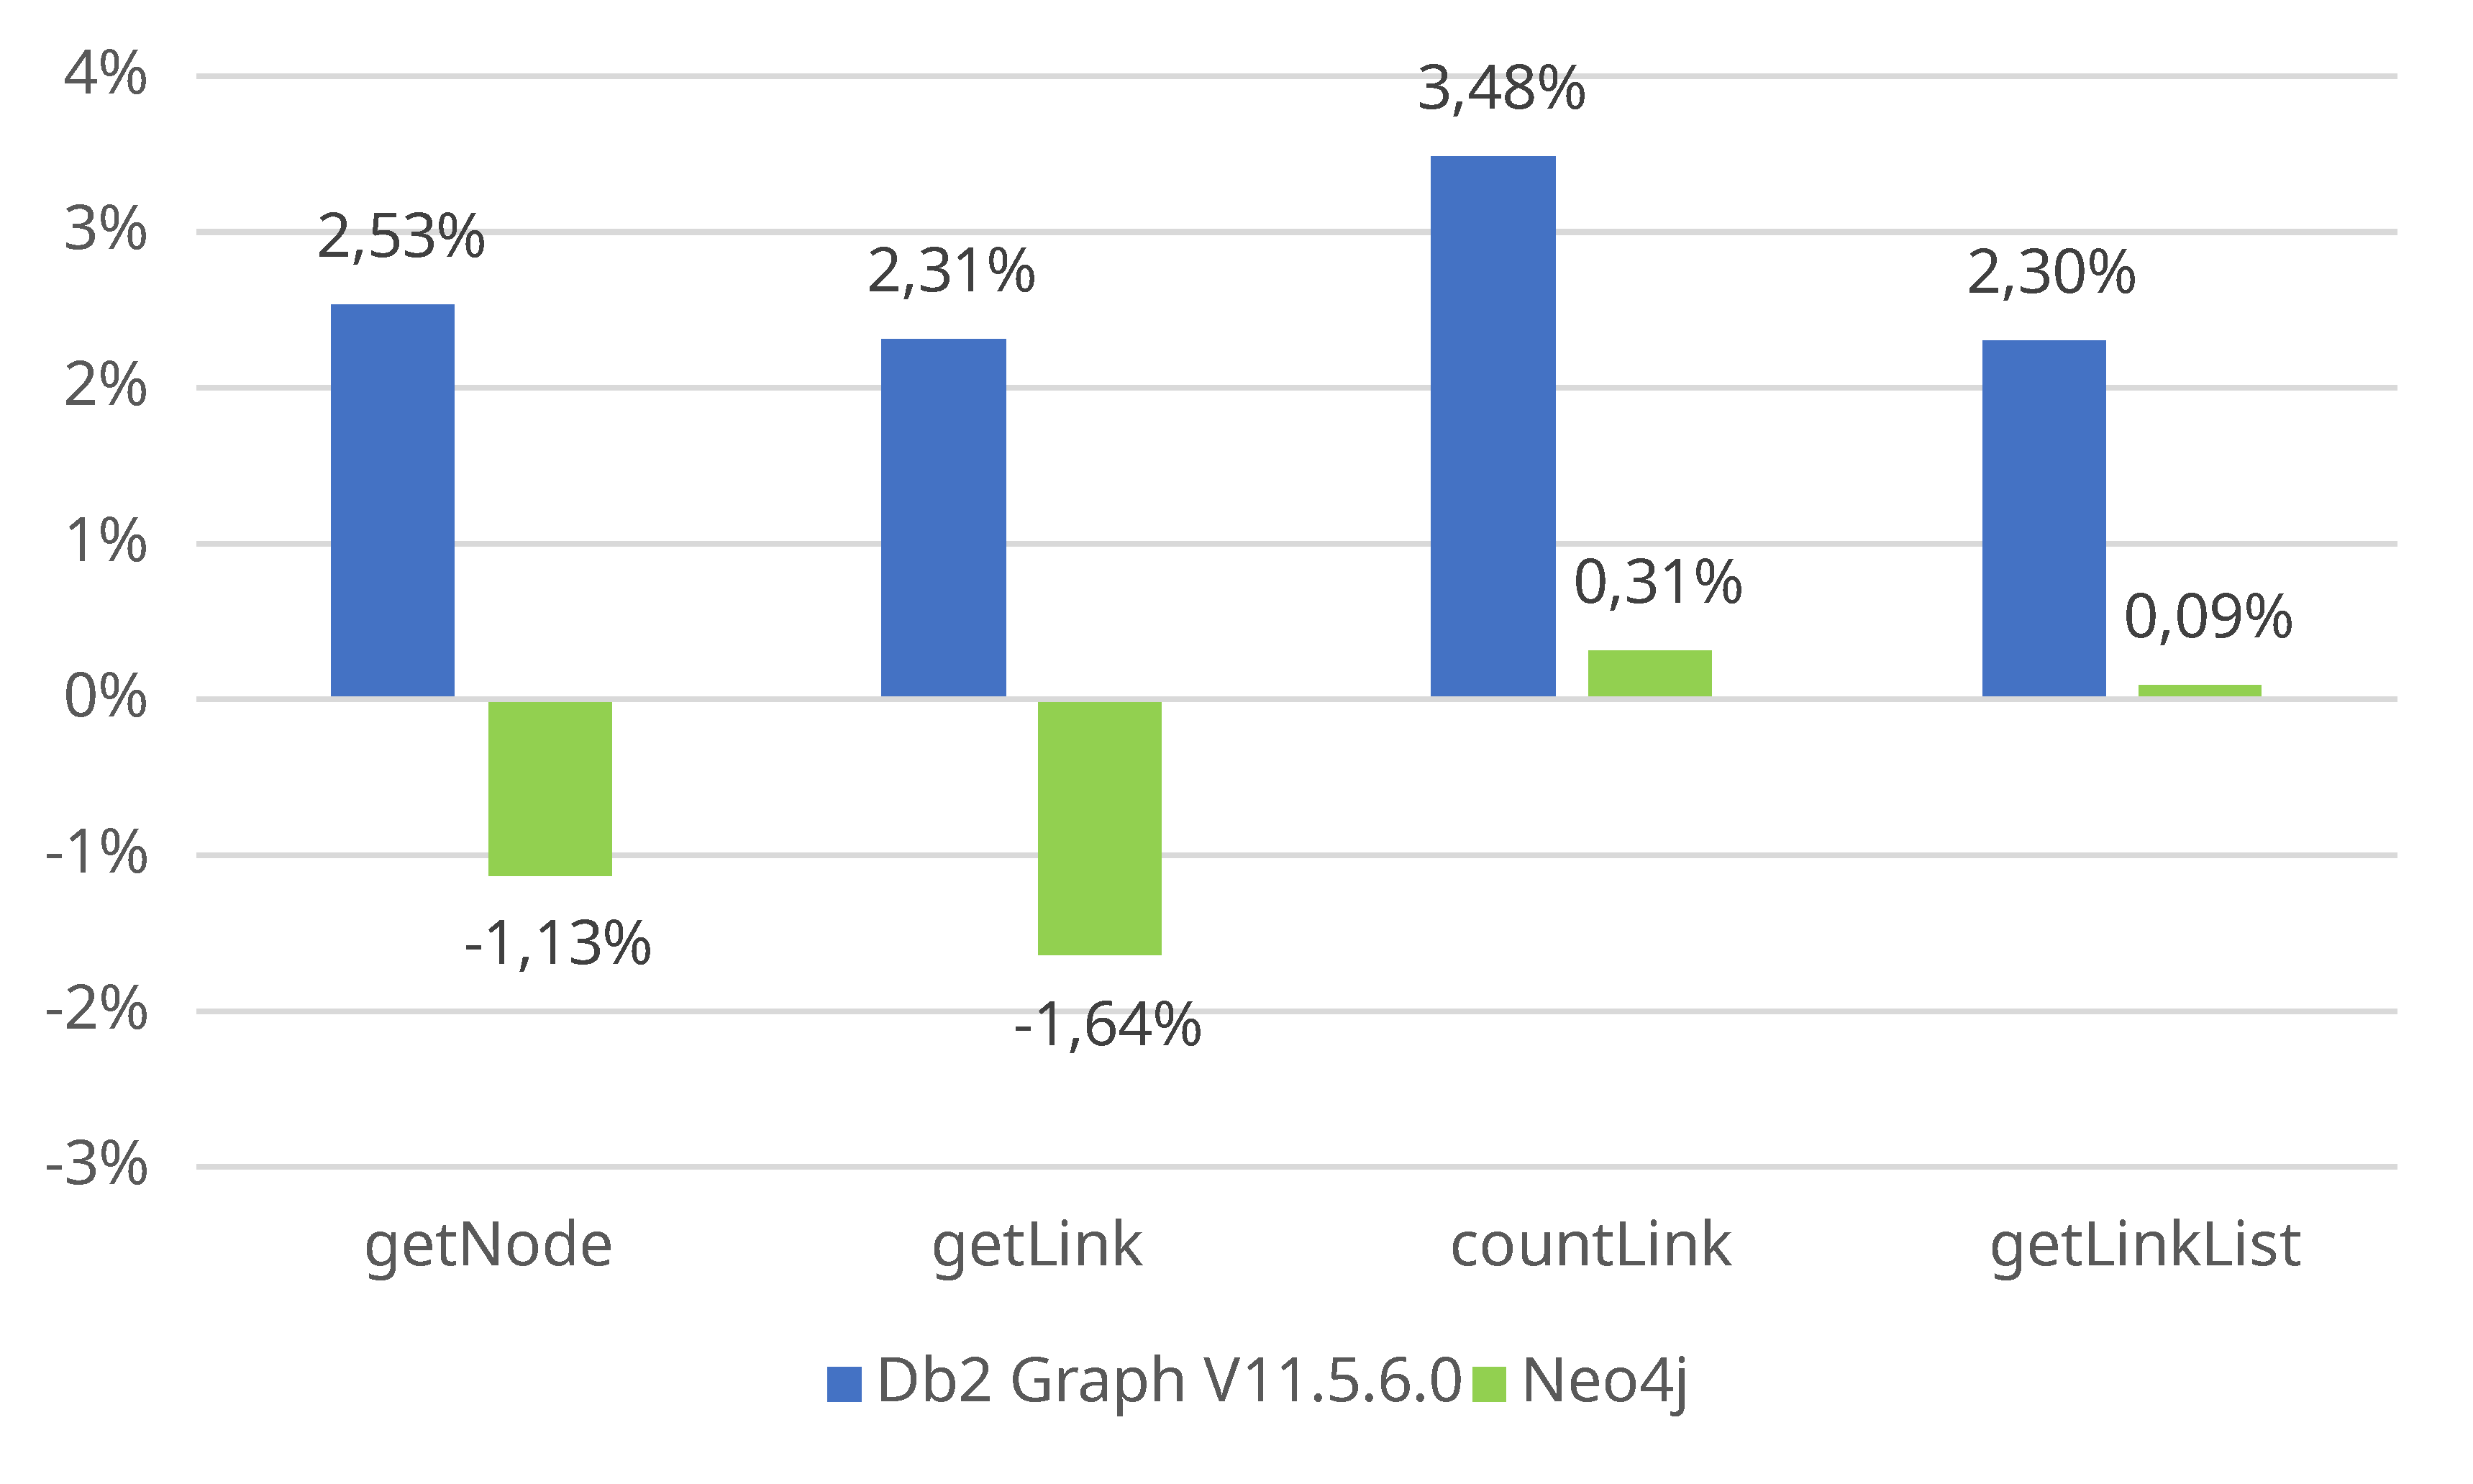
\includegraphics[width=\textwidth]{images/diagramme/difference_durchsatz_real_10m_vs_100m.pdf}
    \caption{Unterschied Durchsatz Linkbench-10M vs. Linkbench-100M (Real)}
    \label{fig:durchsatz:10m_vs_100m:real}
    \vspace{1em}
    \textit{Bei den hier abgebildeten Werten für getLinkList, handelt es sich um Werte, die mit einem Range-Limit von 100 erzielt werden.}
\end{figure}

Die in \autoref{fig:durchsatz:10m_vs_100m:real} abgebildeten Ergebnisse überraschen hingegen. Die Ergebnisse für Neo4j bewegen sich hier bei \texttt{getNode} und \texttt{getLink} im negativen Bereich. Dies bedeutet, dass für Neo4j bei diesen Operationen in \nameref{ergebnisse:100m_real} ein höherer Durchsatz erzielt werden konnte, als bei dem kleineren Datensatz in \nameref{ergebnisse:10m_real}, was der bereits zuvor geäußerten These, dass größere Datensätze einen geringeren Durchsatz beziehungsweise eine geringere Performance aufweisen, widerspricht. Auch gibt es bei den Messungen keinerlei Anhaltspunkte, warum dieses Phänomen bei Neo4j auftritt. Alle anderen Werte von Neo4j und Db2 Graph V11.5.6.0 weisen hingegen positive Performance-Verschlechterungen auf.

Bezüglich der Höhe der Abweichungen kann aus \autoref{fig:durchsatz:10m_vs_100m:real} abgeleitet werden, dass Db2 Graph mit Abweichungen zwischen 2,3 \% und 3,48 \% eine höhere Abweichung aufweist als Neo4j, welche sich im Bereich von 0,09 \% bis (-)1,64 \% bewegt. 

\section{Ressourcenauslastung}
\label{auswertung:ressourcenauslastung}

Im Rahmen dieses Kapitels werden einige NMON-Statistiken zur Ressourcenauslastung ausgewertet. Dabei wird die CPU- und IO-Aus\-last\-ung genauer untersucht und die darin erkennbaren Trends und Unterschiede zwischen den Datenbanksystemen angesprochen. 

Ziel dieses Abschnitts ist es dabei die Ressourcenauslastung der Datenbanksysteme miteinander zu Vergleichen und möglicherweise einen Hinweis darauf zu finden, warum der Performance-Unterschied zwischen Db2 Graph Beta 3 und V11.5.6.0 mit einem Unterschied des Faktors 2,25 derart signifikant ausfällt. 

Für den Vergleich der Datenbanksysteme wird dabei exemplarisch deren Ressourcenauslastung bei der Operation \texttt{getNode} in den Messreihen \nameref{ergebnisse:10m_const} und \nameref{ergebnisse:10m_real} herangezogen. Denn die Abbildung und Auswertung aller 52 Statistiken, die bei der Performance-Analyse durch das Werkzeug NMON aufgezeichnet werden, wäre hier aufgrund des Umfangs nicht zielführend. Alle Statistiken, die im Rahmen der Arbeit aufgezeichnet werden, werden allerdings als NMON-Dateien dem digitalen Anhang der Arbeit beigelegt, sodass alle erzielten Statistiken einsehbar sind.

Bei der Auswertung der Statistiken gilt es allerdings zu beachten, dass die CPU-Auslastung und Anzahl an IO-Ope\-ra\-ti\-on\-en (Disk xfers) pro Sekunde, die von den Abbildungen dieses Abschnitts aufgeführt werden, immer die Auslastung der ganzen Maschine, in der die Messungen stattfinden, wiedergeben. So gilt es dabei auch immer im Auge zu behalten, dass beispielsweise das Betriebssystem selbst und andere kleinere Server-Prozesse ebenfalls geringfügig etwas zur CPU- und IO-Aus\-last\-ung beitragen.  

\subsection{Linkbench-Const-10M}
\label{auswertung:ressourcenauslastung:const}
Bei der Auswertung der Ressourcenstatistiken dieser Messreihe kann mit Hinblick auf diese identifiziert werden, dass die CPU-Auslastung bei Neo4j (\autoref{fig:nmon:10m:const:neo4j}) am höchsten ist, gefolgt von Db2 Graph Beta 3 (\autoref{fig:nmon:10m:const:beta3}) und mit größerem Abstand Db2 Graph V11.5.6.0 (\autoref{fig:nmon:10m:const:ga}). 

Dabei fällt auf, dass der Unterschied bei der CPU-Auslastung zwischen Neo4j und Db2 Graph Beta 3 mit ca. 5 bis 7 \% eher geringer ausfällt, während der Unterschied zwischen Beta 3 und V11.5.6.0 ca. 30 \% umfasst. Dies scheint allerdings ungefähr zu den Beobachtungen in \compref{auswertung:einordnung} zu passen, bei der Beta 3 die 2,25-fache Performance von V11.5.6.0 aufweist. Schließlich weist Beta 3 mit ca. 69 \% gegenüber der rund 39 \% von V11.5.6.0 auch nahezu die doppelte Ressourcenauslastung auf.

\begin{figure}[!ht]
    \centering
    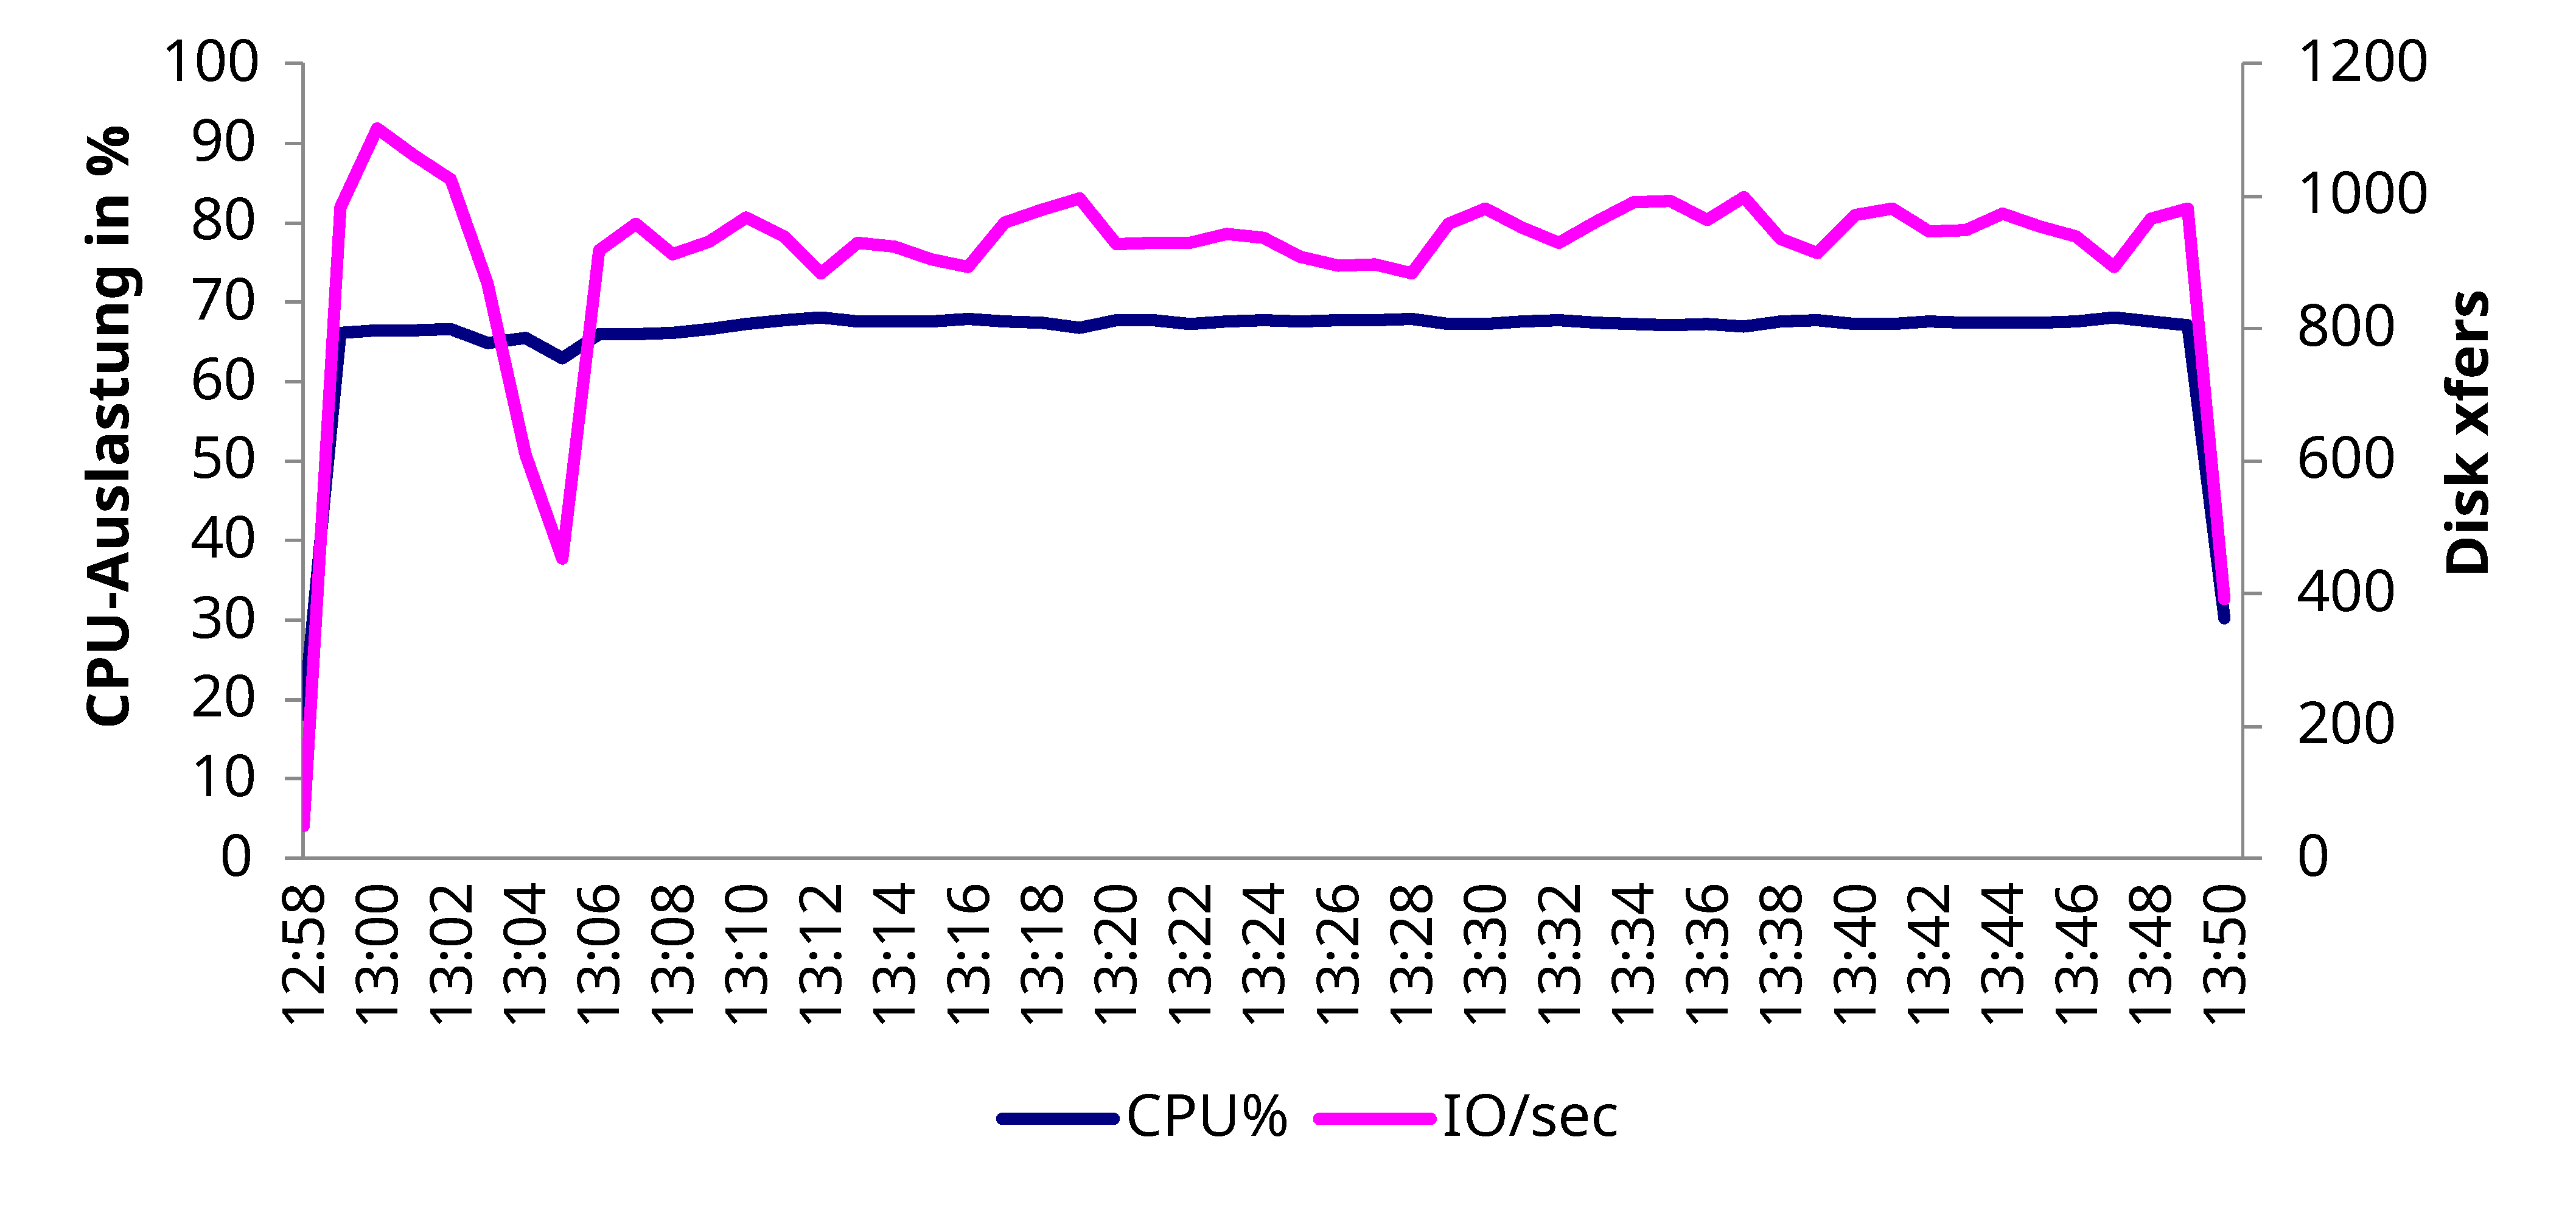
\includegraphics[width=\textwidth]{images/stats/linkbench-10m-const_beta3.pdf}
    \caption{Linkbench-Const-10M Auslastung Db2 Graph Beta 3 getNode}
    \label{fig:nmon:10m:const:beta3}
\end{figure}

Allgemein kann angemerkt werden, dass alle Statistiken eine konstante CPU-Auslastung über den jeweiligen Messzeitraum aufweisen. So zeigt beispielsweise die Aufzeichnung für Neo4j (\autoref{fig:nmon:10m:const:neo4j}) eine andauernde CPU-Auslastung von ca. 76 \% über den Messzeitraum an, bis auf den Beginn und das Ende der Aufzeichnung. Db2 Graph Beta 3 und V11.5.6.0 weisen in ihren jeweiligen Statistiken ein ähnlich konstantes Niveau der CPU-Auslastung auf. 

Wird statt der CPU-Auslastung die Anzahl an IO-Ope\-ra\-ti\-on\-en pro Sekunde in den Ressourcenstatistiken der Datenbanksysteme untersucht, so fällt auf, dass sich die Skalen und Werte der IO-Aus\-last\-ung (Disk xfers) in \autoref{fig:nmon:10m:const:beta3}, \ref{fig:nmon:10m:const:neo4j} und \ref{fig:nmon:10m:const:ga} erheblich unterscheiden. Während bei Db2 Graph V11.5.6.0 ca. 3.700 Read- oder Write-Ope\-ra\-ti\-on\-en pro Sekunde auf den Festplattenspeicher durchgeführt werden, sind es bei Neo4j lediglich 2,5 bis 5. 

\begin{figure}[!ht]
    \centering
    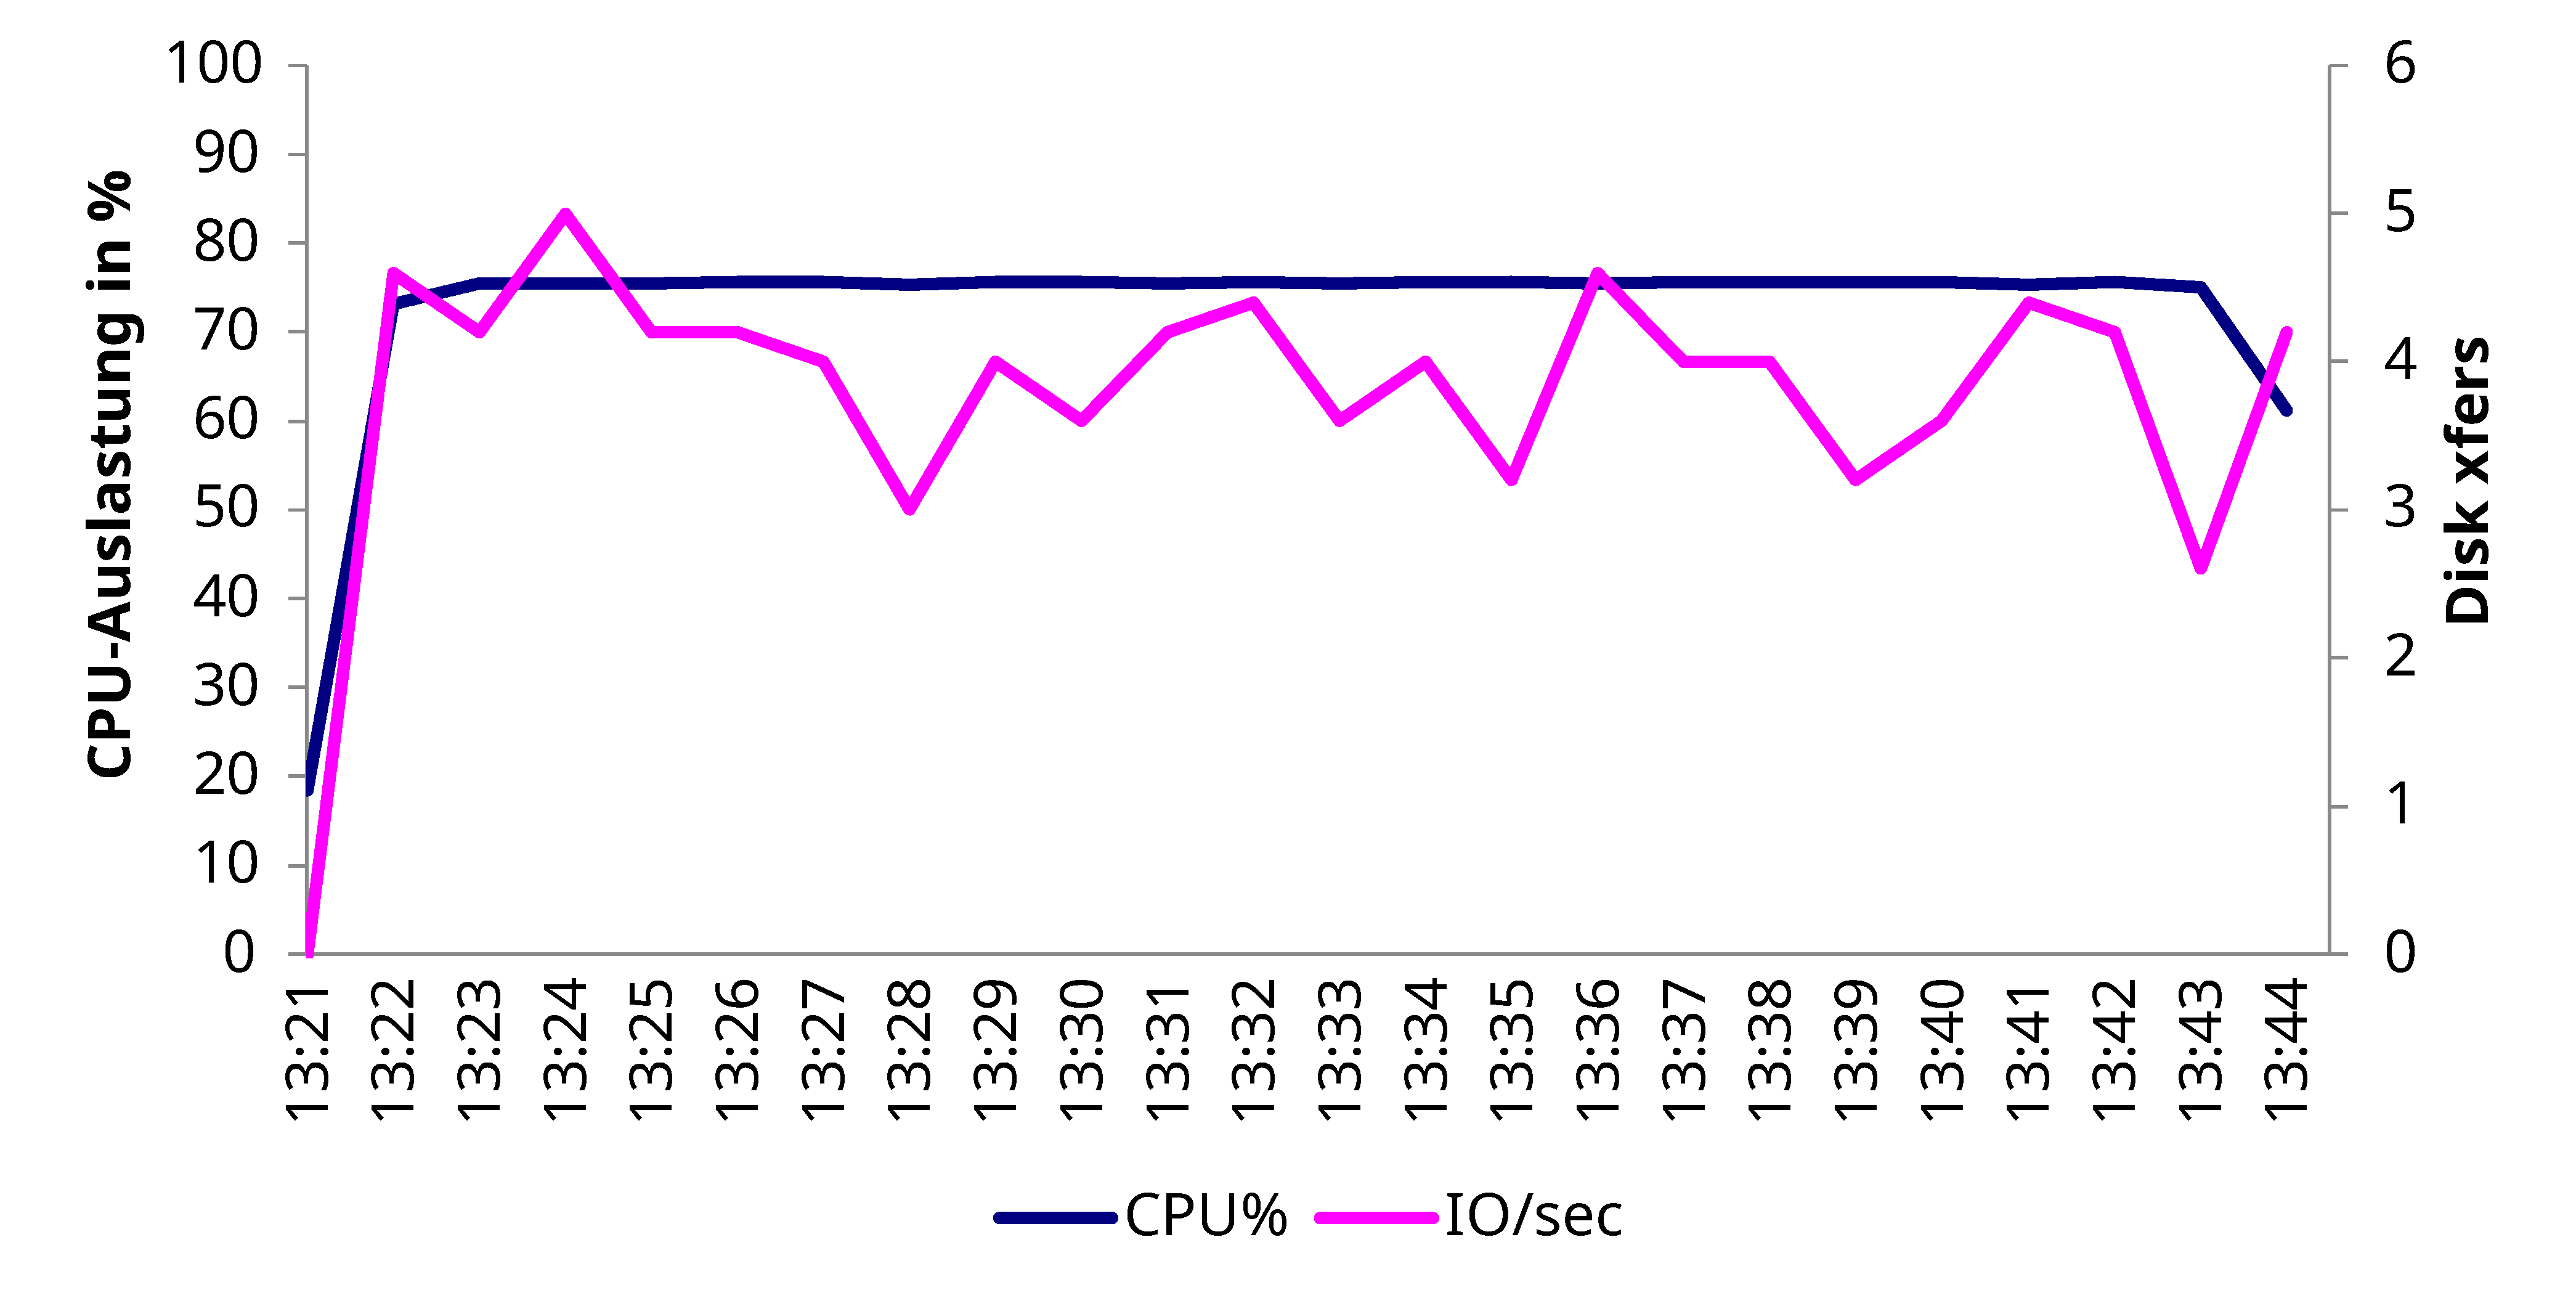
\includegraphics[width=\textwidth]{images/stats/linkbench-10m-const_neo4j.pdf}
    \caption{Linkbench-Const-10M Auslastung Neo4j getNode}
    \label{fig:nmon:10m:const:neo4j}
\end{figure}

\begin{figure}[!ht]
    \centering
    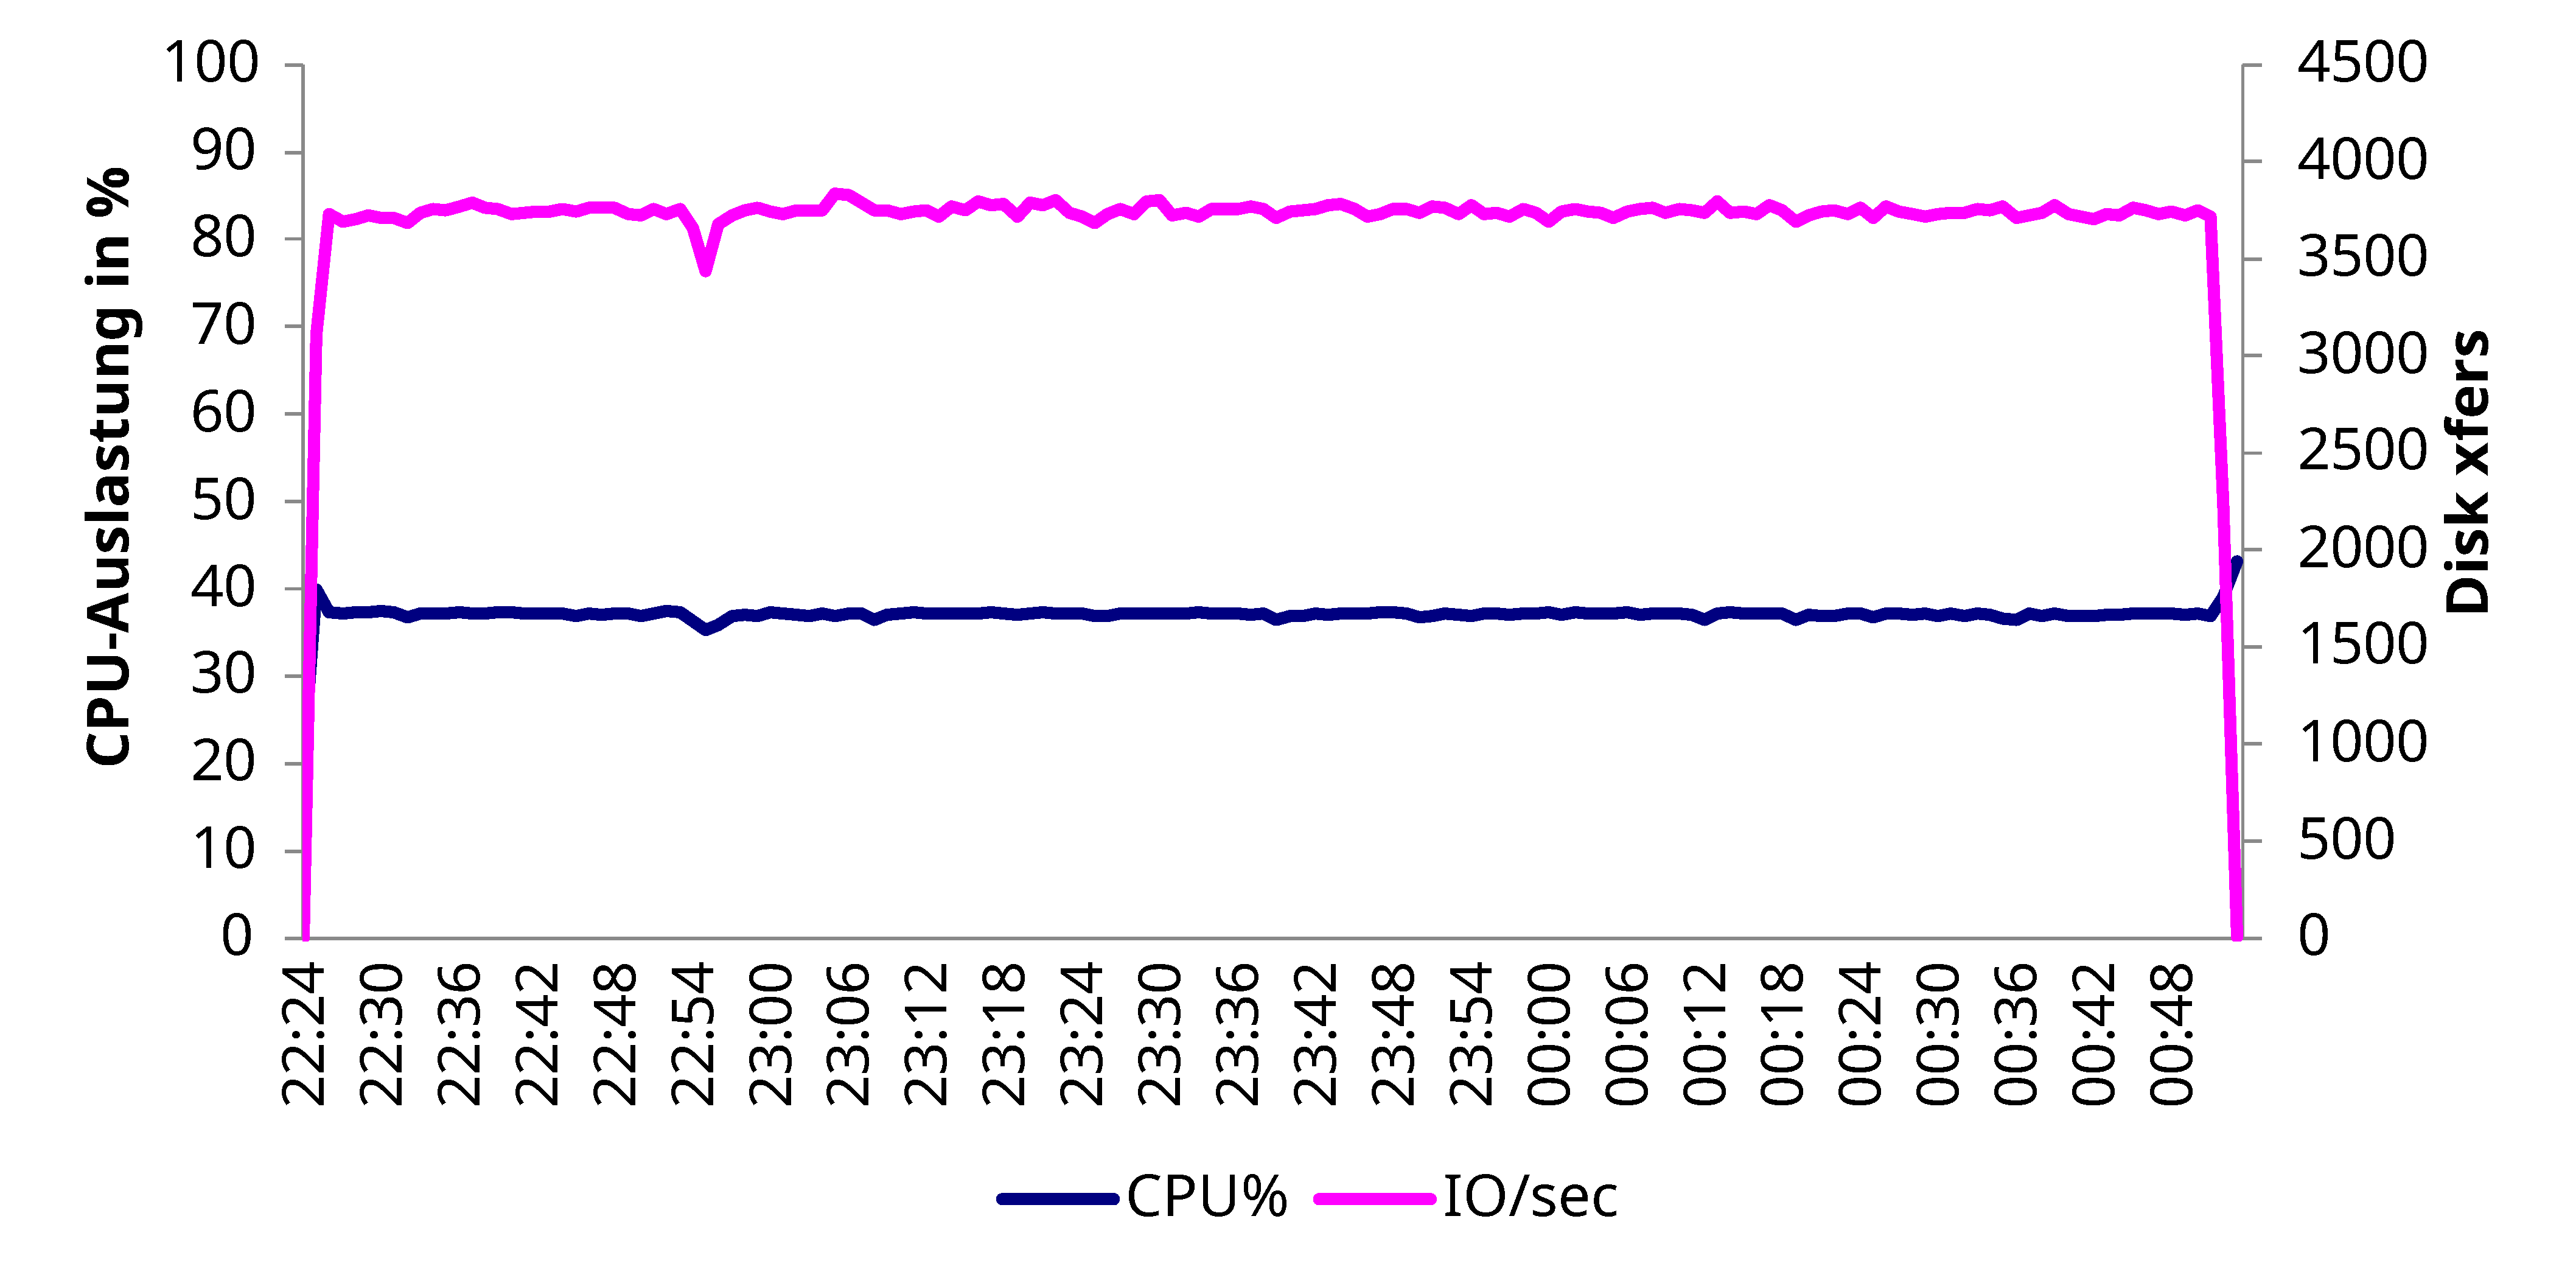
\includegraphics[width=\textwidth]{images/stats/linkbench-10m-const_ga.pdf}
    \caption{Linkbench-Const-10M Auslastung Db2 Graph V11.5.6.0 getNode}
    \label{fig:nmon:10m:const:ga}
\end{figure}

Db2 Graph Beta 3 bewegt sich hingegen mit durchschnittlich ca. 900 IO-Ope\-ra\-ti\-on\-en pro Sekunde im Mittelfeld. Damit liegt Beta 3 zwar unterhalb von V11.5.6.0, weist allerdings immer noch mehr als das Hundertfache der durchschnittlichen IO-Ope\-ra\-ti\-on\-en pro Sekunde von Neo4j auf. Die signifikant geringere IO-Aus\-last\-ung könnte sich damit erklären lassen, dass Neo4j scheinbar ein erheblich aggressiveres Caching betreibt als Db2, auf das sich die beiden Db2 Graph Versionen verlassen. 

\subsection{Linkbench-Real-10M}
\label{auswertung:ressourcenauslastung:real}
Bei den beiden im Rahmen dieser Messreihe aufgezeichneten Ressourcenstatistiken fällt bereits bei der ersten Begutachtung auf, dass die Statistiken für Db2 Graph V11.5.6.0 und besonders Neo4j über weitaus weniger Datenpunkte verfügen als die Abbildungen aus dem vorausgegangen \autoref{auswertung:ressourcenauslastung:const}. Dies ist dabei auf den Umstand zurückzuführen, dass die Messreihen, die auf Basis eines real verteilten Datensatzes operieren, eine niedrigere Request-Anzahl pro Messung aufweisen als bei Messreihen mit konstant verteilten Datensätzen. Dies hat zur Folge, dass Neo4j und Db2 Graph V11.5.6.0 weniger Zeit für die Durchführung der Messungen benötigen. Der kleinere Messzeitraum sorgt dabei wiederum dafür, dass NMON weniger Datenpunkte für die Ressourcenstatistiken sammelt. Schließlich legt NMON während allen Messungen lediglich einen Datenpunkt pro Minute an. 

Bei der Analyse der CPU-Auslastung fällt auf, dass Db2 Graph V11.5.6.0 (\autoref{fig:nmon:10m:real:ga}) und Neo4j (\autoref{fig:nmon:10m:real:neo4j}) mit durchschnittlich ca. 39 \% und 76 \% ähnliche Werte wie im vorausgegangen \autoref{auswertung:ressourcenauslastung:const} darlegen. So verursacht Neo4j über seinen Messzeitraum eine höhere CPU-Auslastung als V11.5.6.0 in seinem.   

Des Weiteren weisen beide Datenbanksysteme auch über den gesamten Verlauf der Messung ein Niveau auf, das sie bis auf die erste Messung konstant halten. Wobei es hierbei zu beachten gilt, dass für diese Erhebung bei Neo4j lediglich vier Datenpunkte herangezogen werden.

\begin{figure}[!ht]
    \centering
    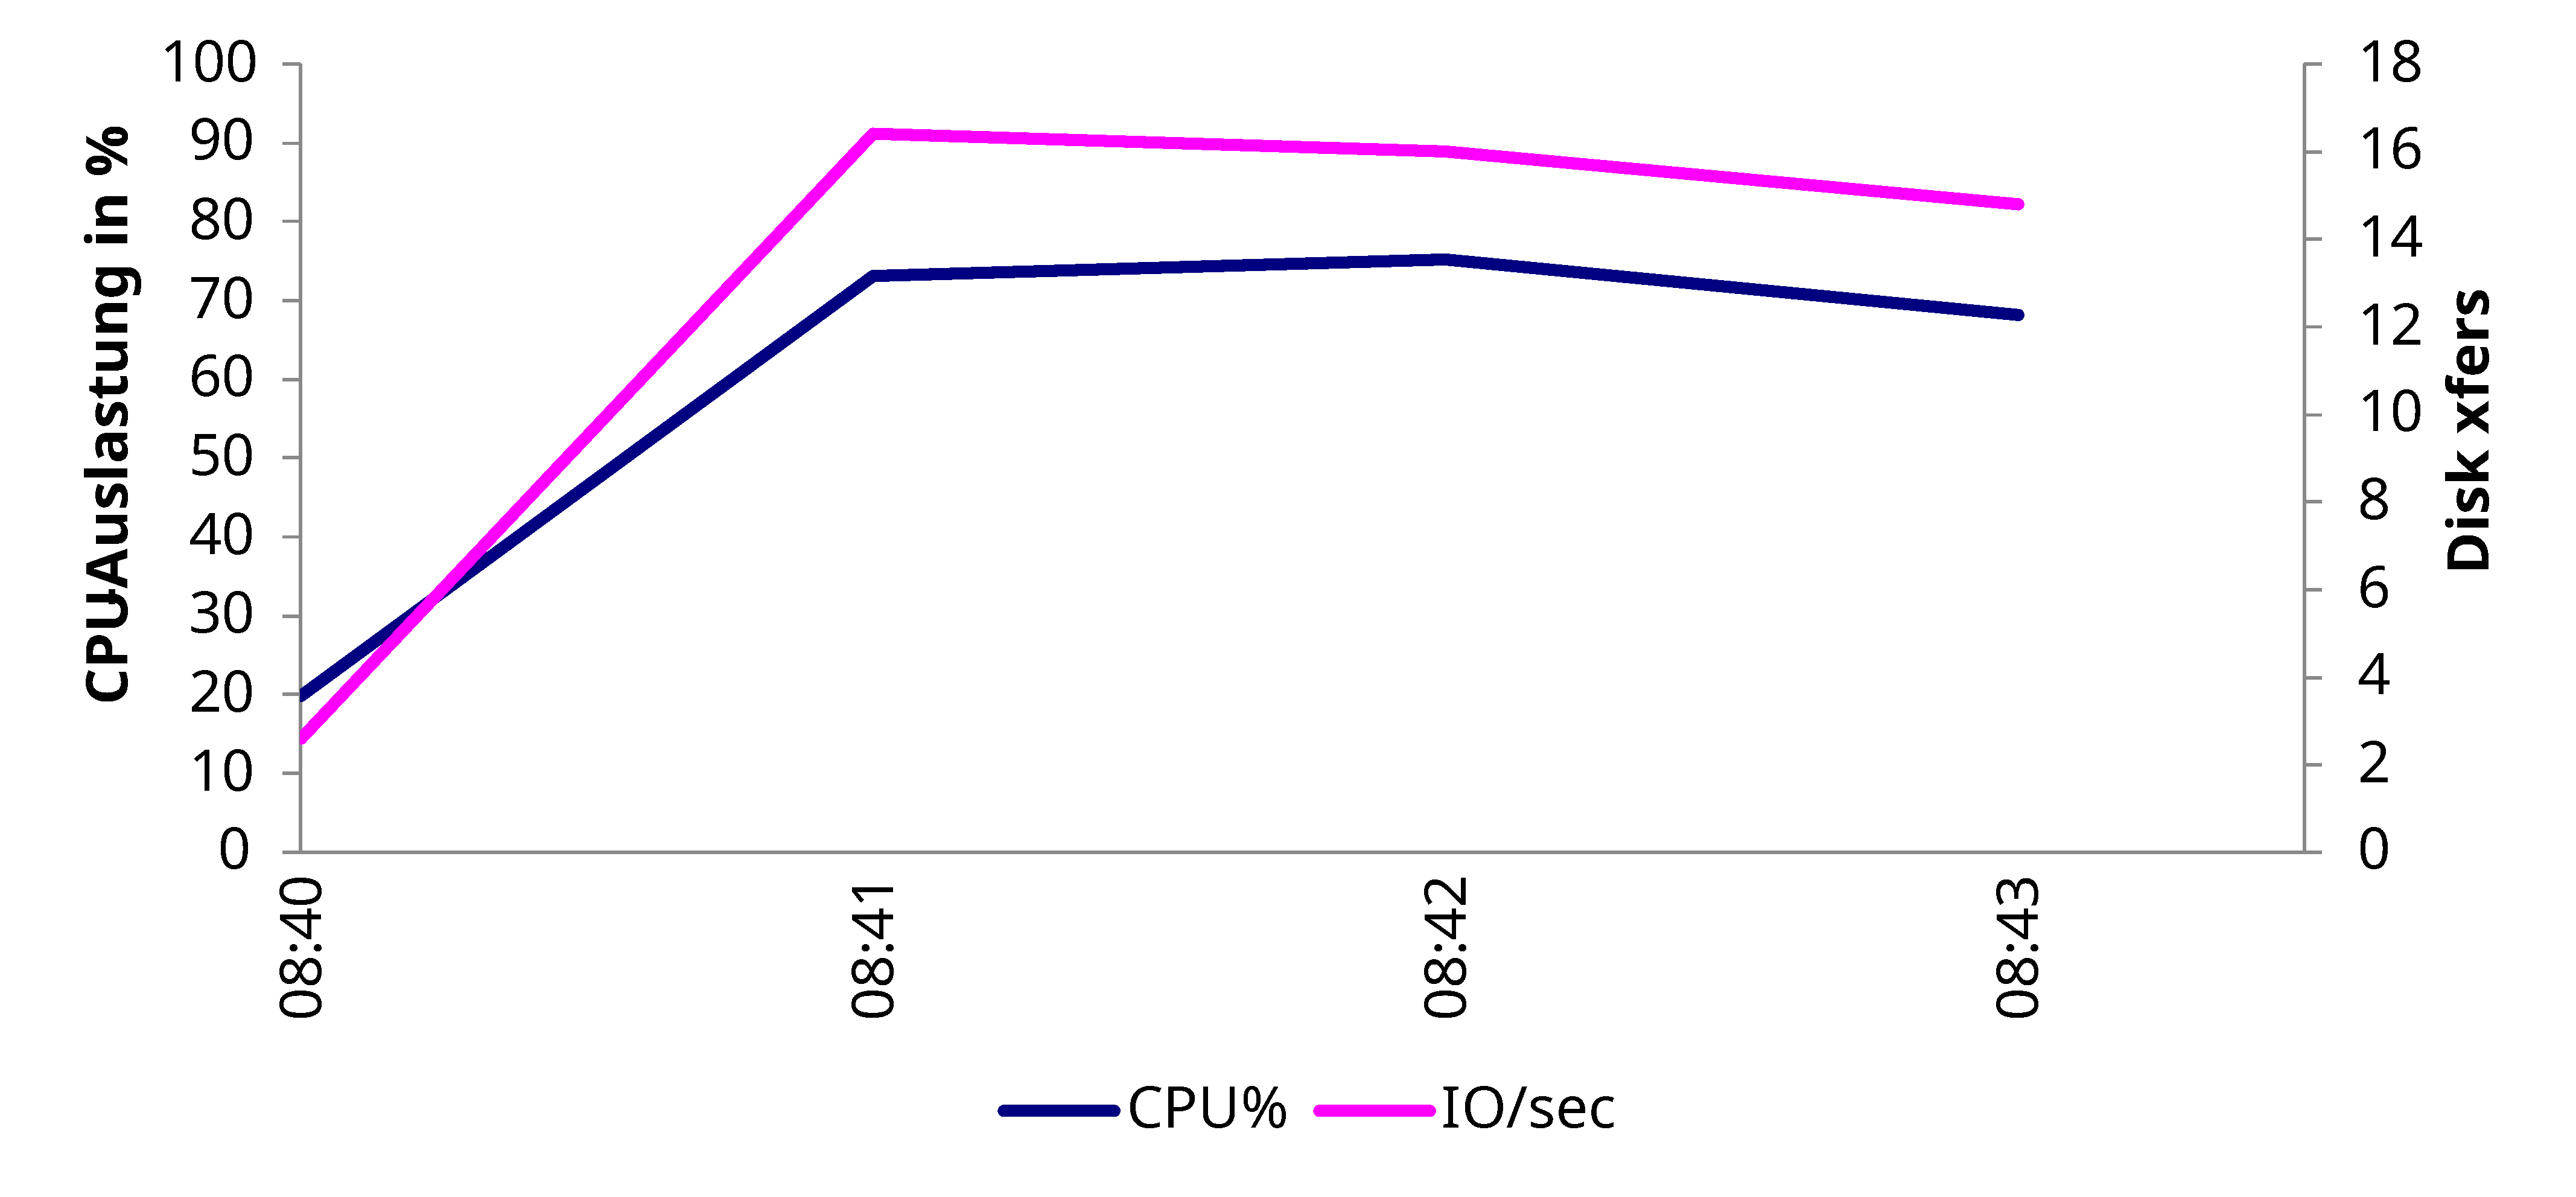
\includegraphics[width=\textwidth]{images/stats/linkbench-10m-real_ga.pdf}
    \caption{Linkbench-Real-10M Auslastung Db2 Graph V11.5.6.0 getNode}
    \label{fig:nmon:10m:real:ga}
\end{figure}

\begin{figure}[!ht]
    \centering
    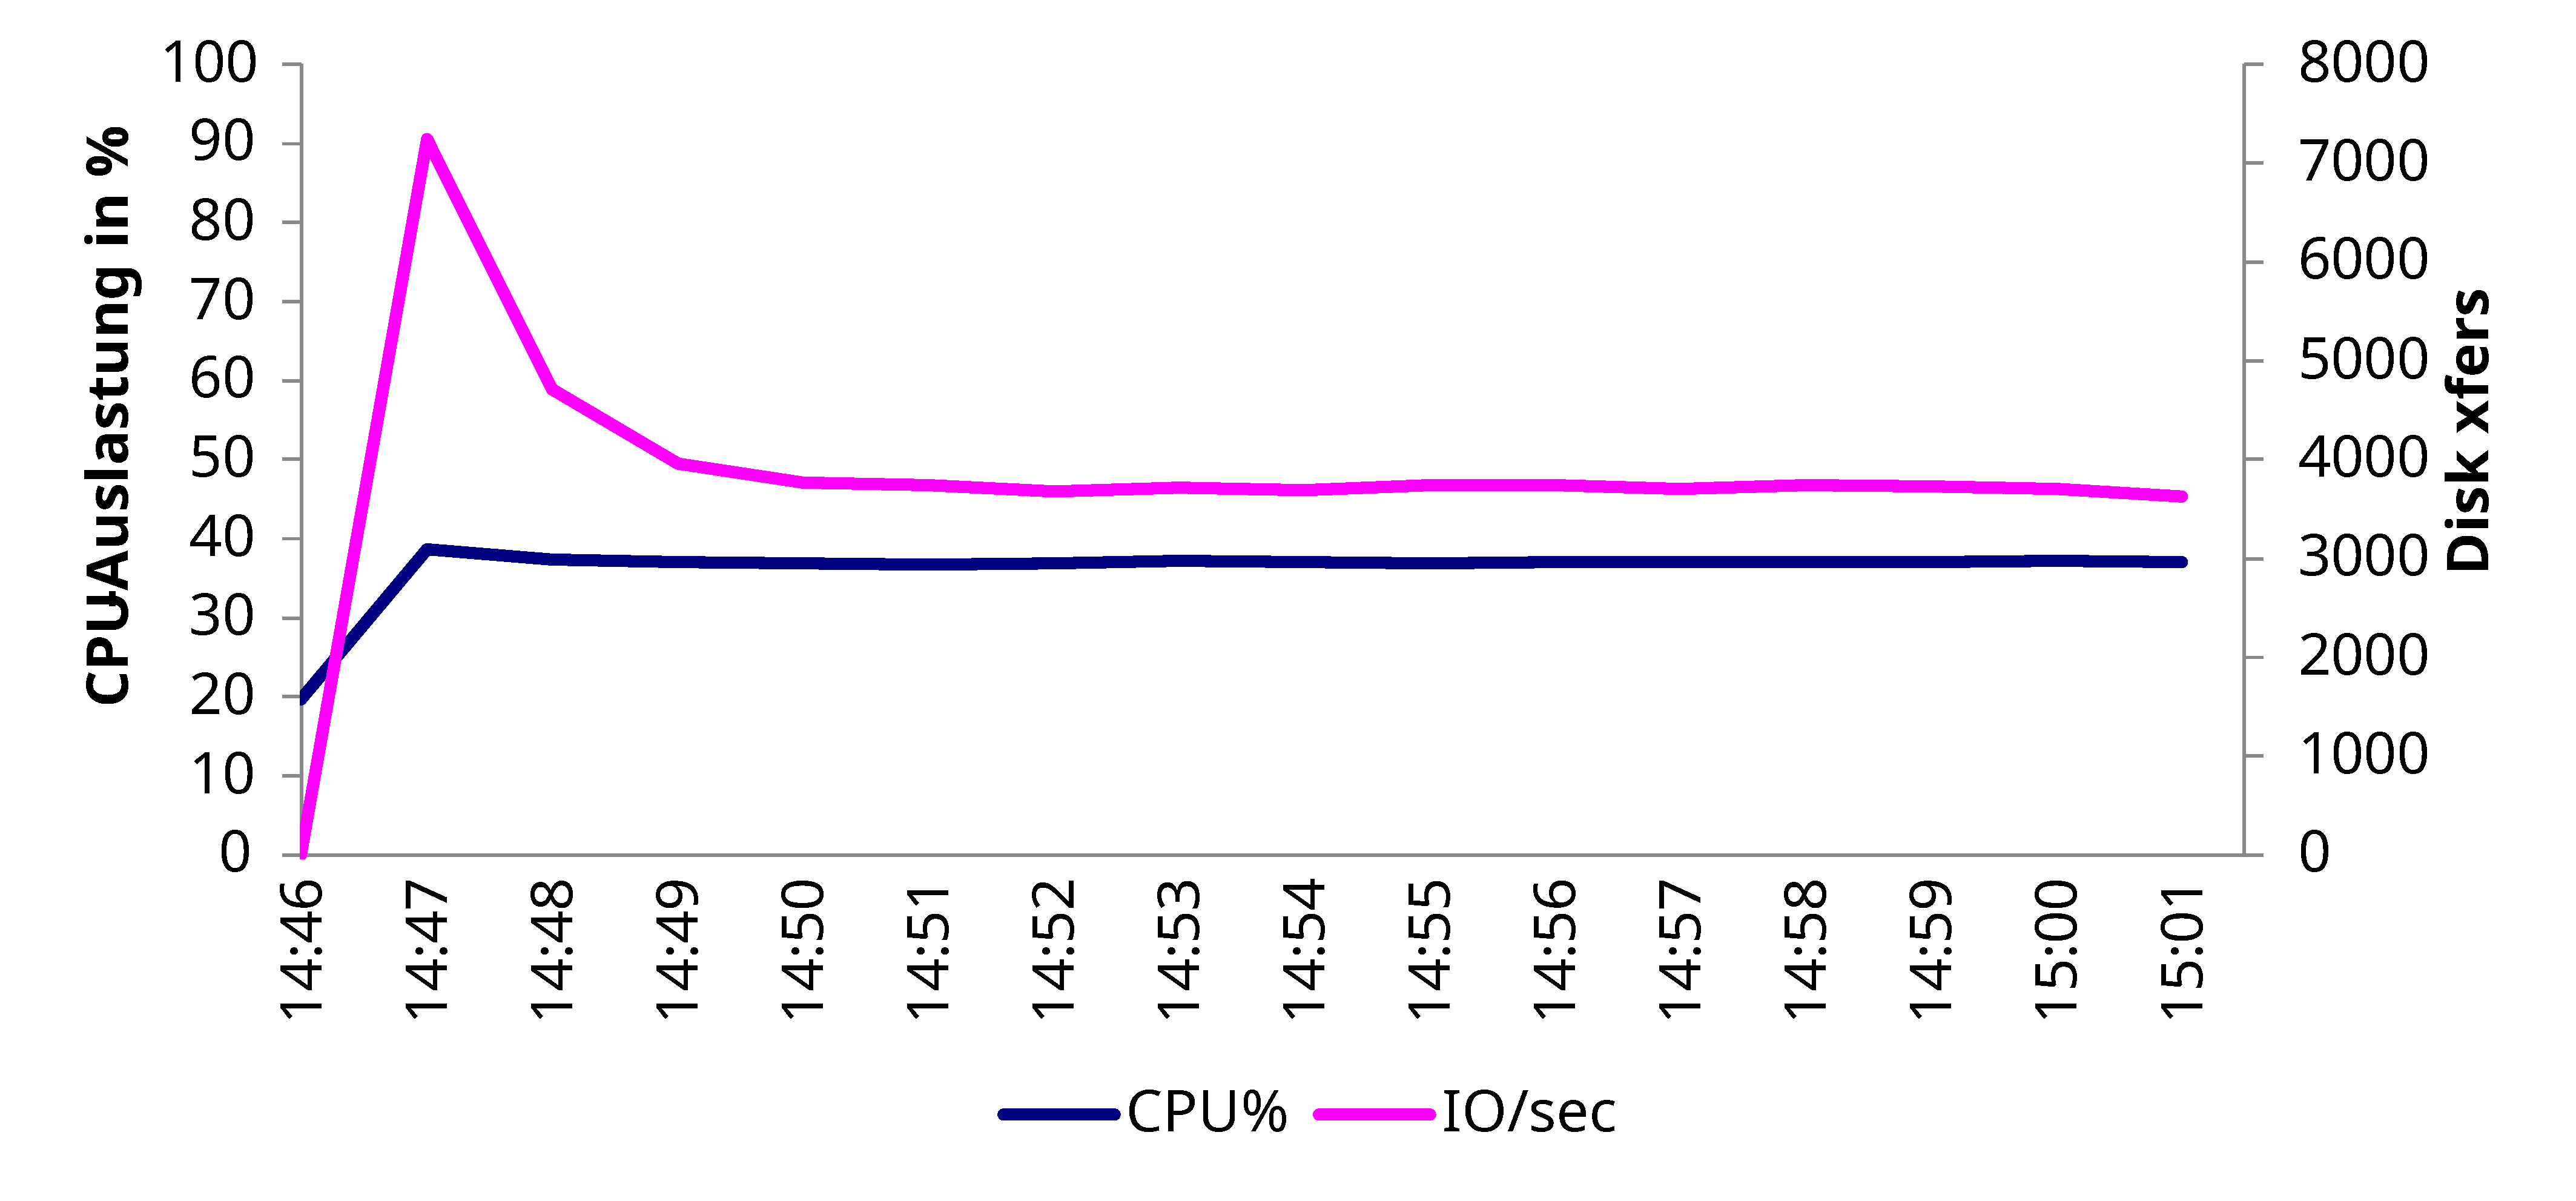
\includegraphics[width=\textwidth]{images/stats/linkbench-10m-real_neo4j.pdf}
    \caption{Linkbench-Real-10M Auslastung Neo4j getNode}
    \label{fig:nmon:10m:real:neo4j}
\end{figure}

Bei der IO-Auslastung hingegen kann bei Db2 Graph V11.5.6.0 (\autoref{fig:nmon:10m:real:ga}) zu Beginn der Messung eine signifikante Spitze um 14:47 identifiziert werden. An diesem Punkt steigt die Anzahl an IO-Operationen (Disk xfers) kurzzeitig auf mehr als 7.000 pro Sekunde. Anschließend flacht die IO-Auslastung wieder auf die aus \autoref{auswertung:ressourcenauslastung:const} bekannten ca. 3.900 IO-Operationen pro Sekunde ab und hält diese bis zum Ende der Messung.

Die IO-Auslastung ist laut \autoref{fig:nmon:10m:real:neo4j} auch im Kontext dieser Messreihe, mit im Maximalfall ca. 16 IO-Operationen pro Sekunde, außergewöhnlich niedrig. Schließlich gilt es dabei zu beachten, dass auch die Read- und Write-Operationen auf den Festplattenspeicher von anderen Anwendungs- und System-Prozessen in der Statistik mit erfasst werden. Die geringe IO-Auslastung bei Neo4j unterstützt dabei die in \autoref{auswertung:ressourcenauslastung:const} aufgestellte Hypothese, dass Neo4j scheinbar ein weitaus aggressiveres Caching als die Db2 Graph Versionen betreibt.

\section{SQL-Anweisungen}
\label{sql}
In diesem Abschnitt werden die von Db2 Graph Beta 3 und V11.5.6.0 generierten und an Db2 gesendeten SQL-Anweisungen miteinander verglichen und analysiert. Dieser Schritt wird hierbei mit der Absicht durchgeführt, eine Erklärung für den in \autoref{auswertung:einordnung} beschriebenen Performance-Unterschied zwischen den beiden Db2 Graph Versionen zu finden. Schließlich ist die Performance von V11.5.6.0  deutlich geringer als bei Beta 3, bei der es sich eigentlich um die ältere und weniger optimiertere Version von Db2 Graph handelt. Dafür wird in diesem Abschnitt zuerst die Struktur der SQL-Anweisungen verglichen und anschließend kurz die Performance. 

\subsection{Struktur}
\label{sql:struktur}
Um die von den Db2 Graph Versionen generierten SQL-Anweisungen zu erhalten, die an Db2 gesendet werden, wird Db2 so konfiguriert, dass diese alle empfangenen SQL-Anweisungen mit Bezug zur \texttt{linkdb0}-Datenbank aufzeichnet. So können die Gremlin-Queries per Gremlin-Console an die beiden Db2 Graph Versionen gesendet werden, während Db2 die bei der Verarbeitung dieser Queries empfangenen SQL-Anweisungen protokolliert. Dadurch lassen sich die protokollierten SQL-Anweisungen jeweils einer entsprechenden Gremlin-Query zuordnen. Die protokollierten SQL-Anweisungen und ihre entsprechende Gremlin-Query werden dabei in \autoref{src:sql_getnode} (\texttt{getNode}), \autoref{src:sql_getlink} (\texttt{getLink}), \autoref{src:sql_countlink} (\texttt{countLink}) und \autoref{src:sql_getlinklist} (\texttt{getLinkList}) dargestellt.

Werden die bei \texttt{getNode} und \texttt{getLink} erzeugten SQL-Anweisungen miteinander verglichen,  stechen dort lediglich kleinere Unterschiede zwischen Beta 3 und V11.5.6.0 heraus. So nutzt die von Beta 3 erzeugte SQL-Anweisung mit \texttt{*} eine Wildcard, statt einer expliziten Spezifikation der abgefragten Spalten wie bei V11.5.6.0. Dies dürfte allerdings -- wenn überhaupt -- einen vernachlässigbaren Einfluss auf die Verarbeitungszeit der Anfrage haben.

\begin{lstlisting}[caption={Generierter SQL-Code getNode},label=src:sql_getnode,language=SQL]
/* Gremlin-Query */
g.V()
 .hasLabel("NODETABLE")
 .has("ID", <NODE_ID>);

-- Db2 Graph Beta 3
SELECT * FROM "LINKDB0"."NODETABLE" WHERE "ID" = <NODE_ID>;

-- Db2 Graph V11.5.6.0
SELECT "ID", "VERSION", "TIME", "ID", "DATA", "TYPE" FROM "LINKDB0"."NODETABLE" WHERE "ID" = <NODE_ID>;
\end{lstlisting}

\begin{lstlisting}[caption={Generierter SQL-Code getLink},label=src:sql_getlink,language=SQL]
/* Gremlin-Query */
g.E()
 .hasLabel("LINKTABLE")
 .has("LINK_TYPE", <LINK_TYPE>)
 .has("ID1", <NODE_ID1>)
 .has("ID2", P.within(<NODE_ID2s>))

-- Db2 Graph Beta 3
SELECT * FROM "LINKDB0"."LINKTABLE" WHERE "LINK_TYPE" = <LINK_TYPE> AND "ID1" = <NODE_ID1> AND "ID2" IN (VALUES <NODE_ID2_0>, <NODE_ID2_1>, <...>);

-- Db2 Graph V11.5.6.0
SELECT "ID1", "ID2", "LINK_TYPE", "ID1", "ID2", "VISIBILITY","LINK_TYPE", "DATA", "ID2", "ID1", "VERSION", "TIME" FROM "LINKDB0"."LINKTABLE" WHERE "LINK_TYPE" = <LINK_TYPE> AND "ID1" = <NODE_ID1> AND "ID2" IN (VALUES <NODE_ID2_0>, <NODE_ID2_1>, <...>);
\end{lstlisting}

Bei der Untersuchung der von \texttt{countLink} und \texttt{getLinkList} sind jedoch größere Unterschiede erkennbar. So verfügt, wie in \autoref{db2graph:optimierung} erläutert wird, Beta 3 nicht über die Optimierungen \textit{Join Pushdown} und \textit{Limit Pushdown}, was sich im Kontext von \texttt{countLink} (\autoref{src:sql_countlink}) und \texttt{getLinkList} (\autoref{src:sql_getlinklist}) bemerkbar macht. Beta 3 erzeugt und sendet dabei den Aufzeichnungen zu Folge zwei SQL-Anweisungen an Db2, während V11.5.6.0 dazu in der Lage ist, die Logik der Gremlin-Query durch einen (impliziten) Join in eine SQL-Anweisung zu integrieren. Dies sollte sich auf die Performance der Queries auswirken, allerdings, entgegen der in \autoref{ergebnisse} aufgeführten Messergebnisse, zum Vorteil von V11.5.6.0, nicht Beta 3. 

Des Weiteren reflektiert die von Beta 3 erzeugte Anweisung auch nicht die Existenz des Limit-Steps in SQL, da es die Optimierung \textit{Limit Pushdown} nicht beherrscht. Dies dürfte sich allerdings, wie in \autoref{analyse:datensatz} erläutert wird, nicht auf die Performance bei konstant verteilten Datensätzen auswirken. Da, wie in \autoref{analyse:datensatz} ebenfalls beschrieben wird, aufgrund dieser fehlenden Optimierung auch keine Messungen mit Beta 3 und real verteilten Datensätzen durchgeführt werden, sollte dieser Aspekt im Kontext des hier untersuchten Phänomens vernachlässigbar sein. 
\begin{lstlisting}[caption={Generierter SQL-Code countLink},label=src:sql_countlink,language=SQL]
/* Gremlin-Query */
g.V()
 .hasLabel("NODETABLE")
 .has("ID", <NODE_ID>)
 .outE("LINKTABLE")
 .has("LINK_TYPE", <LINK_TYPE>)
 .count()

-- Db2 Graph Beta 3
SELECT * FROM "LINKDB0"."NODETABLE" WHERE "ID" = <NODE_ID>;
SELECT * FROM "LINKDB0"."LINKTABLE" WHERE ("ID1") IN (VALUES (<NODE_ID>)) AND "LINK_TYPE" = <LINK_TYPE>;

-- Db2 Graph V11.5.6.0
SELECT COUNT(*) FROM "LINKDB0"."NODETABLE" AS VT0, "LINKDB0"."LINKTABLE" AS ET1 WHERE VT0."ID" = <NODE_ID> AND ET1."LINK_TYPE" = <LINK_TYPE> AND VT0.ID = ET1.ID1
\end{lstlisting}

\begin{lstlisting}[caption={Generierter SQL-Code getLinkList},label=src:sql_getlinklist,language=SQL]
/* Gremlin-Query */
g.V()
 .hasLabel("NODETABLE")
 .has("ID", <NODE_ID1>)
 .outE("LINKTABLE")
 .has("LINK_TYPE", <LINK_TYPE>)
 .limit(<LIMIT>);

-- Db2 Graph Beta 3
SELECT * FROM "LINKDB0"."NODETABLE" WHERE "ID" = <NODE_ID>;
SELECT * FROM "LINKDB0"."LINKTABLE" WHERE ("ID1") IN (VALUES (<NODE_ID>)) AND "LINK_TYPE" = <LINK_TYPE>;

-- Db2 Graph V11.5.6.0
SELECT ET1."ID1", ET1."ID2", ET1."LINK_TYPE", ET1."ID1", ET1."ID2", ET1."VISIBILITY", ET1."LINK_TYPE", ET1."DATA", ET1."ID2", ET1."ID1", ET1."VERSION", ET1."TIME" FROM "LINKDB0"."NODETABLE" AS VT0, "LINKDB0"."LINKTABLE" AS ET1 WHERE VT0."ID" = <NODE_ID> AND ET1."LINK_TYPE" = <LINK_TYPE> AND VT0.ID = ET1.ID1 FETCH FIRST <LIMIT> ROWS ONLY;
\end{lstlisting}

Abschließend kann zusammengefasst werden, dass auf Basis des hier durchgeführten strukturellen Vergleichs der von Db2 Graph Beta 3 und V11.5.6.0 erzeugten SQL-Anweisungen die folgenden beiden Hypothesen aufgestellt werden können:
\begin{itemize}
    \item \textit{Die SQL-Anweisungen bei getNode und getLink sollten -- wenn überhaupt -- in einem vernachlässigbaren Performance-Unterschied zwischen beiden Db2 Graph Versionen resultieren.}
    \item  \textit{Die SQL-Anweisungen bei countLink und getLinkList sollten sich  positiv auf die Performance von V11.5.6.0 auswirken.}
\end{itemize}

\subsection{Performance}
\label{sql:performance}
Um die Performance der von Db2 Graph erzeugten SQL-Anweisungen zu überprüfen, werden diese mittels des Db2-Werkzeuges \texttt{db2batch} in einer kleinen Messung gebenchmarkt. Anschließend wird überprüft, ob die in \autoref{sql:struktur} aufgestellten Hypothesen in der Praxis zutreffen.

Wie hoch die Verarbeitungszeit der SQL-Anweisungen aus \autoref{src:sql_getnode} bis \ref{src:sql_getlinklist} ist, wird in \autoref{tab:sql_benchmark} dargestellt. Die darin abgebildeten Werte werden mit dem \texttt{db2batch}-Werkzeug auf Basis des konstant verteilten Linkbench-10M Datensatzes ermittelt. Außerdem gilt es zu erwähnen, dass die Werte bei \texttt{countLink} und \texttt{getLinkList} für Db2 Graph Beta 3 in \autoref{tab:sql_benchmark} die addierten Werte beider erzeugten SQL-Anweisungen widerspiegeln. 

Bevor mit der Beurteilung der Werte in \autoref{tab:sql_benchmark} begonnen werden kann, muss darauf hingewiesen werden, dass die in der Tabelle aufgeführten Zeiten nicht mit den im Rahmen der Performance-Analyse ermittelten Latenzen vergleichbar sind. Schließlich liegen bei den Messungen mit dem \texttt{db2batch}-Werkzeug andere Bedingungen vor als bei dem Einsatz von Linkbench. 

\begin{table}[!ht]
    \centering
    \begin{tabular}{l|r|r}
    \hline
    \rowcolor[HTML]{EFEFEF} 
    \multicolumn{1}{c|}{\cellcolor[HTML]{EFEFEF}{\color[HTML]{333333} \textbf{SQL-Anweisung}}} & \multicolumn{1}{c|}{\cellcolor[HTML]{EFEFEF}\textbf{Db2 Graph Beta 3}} & \multicolumn{1}{c}{\cellcolor[HTML]{EFEFEF}\textbf{Db2 Graph V11.5.6.0}} \\ \hline
    getNode & 3,480ms & 3,327ms \\
    getLink & 0,549ms & 0,458ms \\
    countLink & 3,750ms & 0,298ms \\
    getLinkList & 2,526ms & 0,251ms \\ \hline
    \end{tabular}
    \caption{Performance der von Db2 Graph erzeugten SQL-Anweisungen}
    \label{tab:sql_benchmark}
\end{table}

Werden die von \autoref{tab:sql_benchmark} aufgeführten Werte genauer analysiert, so ist erkennbar, dass sich beide der in \autoref{sql:struktur} aufgestellten Hypothesen zu bewahrheiten scheinen. Die Unterschiede zwischen den Werten der beiden Db2 Graph Versionen sind bei \texttt{getNode} und \texttt{getLink} -- wie erwartet -- sehr gering. Sie weichen dabei um ungefähr 0,1 bis 0,2 Millisekunden voneinander ab. Bei \texttt{countLink} und \texttt{getLinkList} herrscht hingegen ein sehr großer Unterschied -- wie ebenfalls erwartet. So wird zur Verarbeitung der beiden Operationen bei Db2 Graph V11.5.6.0 lediglich höchstens ein Zehntel der Zeit benötigt wie bei Beta 3. 

Somit kann in diesem Abschnitt festgestellt werden, dass Db2 Graph V11.5.6.0 den performanteren SQL-Code der beiden Db2 Graph Versionen generiert, was interessanterweise den bei der Performance-Analyse erzielten Ergebnissen in \autoref{ergebnisse} klar widerspricht. Der erzeugte SQL-Code selbst scheint daher nicht der Grund für den großen Unterschied zwischen Beta 3 und V11.5.6.0 zu sein. Allerdings können die in diesem Abschnitt aufgeführten Beobachtungen als Beweis dafür betrachtet werden, dass der Grund für die geringere Performance von Db2 Graph V11.5.6.0, bei konstant verteilten Datensätzen, in der Grapherweiterung selbst liegen muss und nicht bei Db2 als zugrundeliegendes Datenbanksystem. 

Von weiteren Untersuchungen nach der Ursache für den Performance-Unterschied zwischen den Db2 Graph Versionen wird dabei an dieser Stelle allerdings abgesehen, da dies den Umfang der Arbeit und das Thema \textit{Performance-Analyse von Graphdatenbanksystemen -- Vergleich von Db2 Graph und Neo4j} überschreiten würde.